\documentclass[12pt, a4paper]{article}

% set up page margins
\usepackage[a4paper,top=2.5cm,bottom=2.5cm,left=3.5cm,right=2.5cm,headsep=12pt]{geometry}

% set up font
\usepackage[T1]{fontenc}
\usepackage{times}
\usepackage{graphicx}
\usepackage{float}
\usepackage{tikz}
\usetikzlibrary{shapes.geometric, arrows}


% fill in your information here
\newcommand{\university}{
Faculdade de Ciências e Tecnologias
Universidade da Universidade de Coimbra}
\newcommand{\logo}{\includegraphics[width=15cm]{images/UC_H_FundoClaro-verde.png}}
\newcommand{\titletext}{Music Genre Classification - Report}
\newcommand{\authorone}{Jorge Júnior Rodrigues Martins - 2021207642}
\newcommand{\authortwo}{Sancho Amaral Simões - 2019217590}
\newcommand{\professor}{Professor César Teixeira}
\newcommand{\dateinfo}{\today} % use today's date

\begin{document}

% insert a cover page
\begin{titlepage}
\begin{center}
\logo \\
\vspace{2cm} % add some vertical space
{\huge \bf \titletext} \\
\vspace{1cm} % add some vertical space
{\large Phase 1 - Binary Classification with MDC and feature reduction/selection techniques} \\
\vspace{2cm} % add some vertical space
{\large \authorone} \\
{\large \authortwo} \\
\vspace{0.5cm} % add some vertical space
{\large Supervised by: \professor} \\
\vspace{4cm} % add some vertical space
{\large \university} \\
\vspace{3cm} 
{\small Coimbra \dateinfo}
\end{center}
\end{titlepage}

% insert a table of contents
\tableofcontents
\newpage

% insert introduction
\section{Introduction}

Music genre classification is a challenging task in the field of music information retrieval due to the subjective nature of music and the varying characteristics of different musical genres. One of the most commonly used datasets for music genre classification research is the GTZAN dataset. This dataset contains a diverse set of audio recordings representing ten different musical genres, including blues, classical, country, disco, hip-hop, jazz, metal, pop, reggae, and rock.

The GTZAN dataset provides a wide range of features that can be used for music genre classification. These features include time-domain and frequency-domain features, such as Mel Frequency Cepstral Coefficients (MFCCs), spectral contrast, spectral centroid, and spectral roll-off.

To classify the musical genres in the GTZAN dataset, we will apply pattern recognition techniques, including Mahalanobis Distance Classifier (MDC), Linear Discriminant Analysis Fisher (LDA Fisher), and Principal Component Analysis (PCA). These techniques have been widely used in various fields for classification tasks, including music genre classification.

Overall, the present report aims to provide a comprehensive overview of the GTZAN dataset and the pattern recognition techniques used to classify musical genres. We hope that our findings will contribute to the growing body of research on music genre classification and inform the development of more accurate and reliable music genre classifiers in the future.

\newpage
\section{Goal}

The goal of this project is to develop classifiers for genre discrimination using a traditional pattern-recognition pipeline approach. The project aims to explore two scenarios: Scenario A (Binary classification) and Scenario B (Multiclass classification). The dataset used for this project is available at https://www.kaggle.com/datasets/gabrielopecs/gtzan-modified-music-genre-classification and contains 1000 music snippets in ten different genres.

The project will involve splitting the data into two datasets, one for classifier development and the other for testing. The development dataset will be used for training and validation, while the testing dataset will be used for evaluating the classifiers. The data will also be normalized/standardized, and the factors for normalization/standardization will be obtained from the development dataset and applied prospectively in the testing dataset.

The project will also involve feature selection and dimensionality reduction techniques, such as PCA and LDA, to reduce the number of features and improve classifier performance. The classifiers will be designed using the Minimum Distance classifier and Fisher LDA for Scenario A.

The overall goal of the project is to compare the performance of different classifiers and feature selection/reduction techniques in discriminating between different music genres. The results of the project will be presented in this report which includes a detailed analysis of the findings and insights gained through manual inspection of the predictions.
\newpage

\section{GTZAN dataset}

The GTZAN dataset is a collection of 1000 audio clips of 30 seconds each, representing 10 different musical genres. The purpose of the dataset is to facilitate research in the area of music genre classification and other related fields. The dataset was created by George Tzanetakis and Perry Cook in 2002 and has since become a widely used benchmark dataset for evaluating the performance of music genre classification algorithms.

\section*{Musical genres}

The 10 musical genres present in the GTZAN dataset are:

\begin{itemize}
\item Blues
\item Classical
\item Country
\item Disco
\item Hip-hop
\item Jazz
\item Metal
\item Pop
\item Reggae
\item Rock
\end{itemize}

\section*{Features}

The GTZAN dataset comprises 34 distinct features for each audio clip, which can be broadly categorized into three groups: time-domain, frequency-domain, and spectral features. However, the dimension of the feature matrix is much greater than 34 (i.e., 197), as it includes various statistics extracted from each feature, such as mean, median, and so on.

\textbf{Time-domain features:}

\begin{itemize}
\item Zero Crossing Rate (ZCR) - $ZCR = \frac{1}{N-1}\sum_{n=1}^{N-1}|sgn(x[n])-sgn(x[n-1])|$
\item Energy - $E = \sum_{n=1}^{N}x^2[n]$
\item Entropy of Energy (EE) - $EE = -\sum_{i=1}^{M}p(i)\log_2(p(i))$
\item Spectral centroid - $SC = \frac{\sum_{i=1}^{N}f(i)m(i)}{\sum_{i=1}^{N}m(i)}$
\item Spectral spread - $SS = \sqrt{\frac{\sum_{i=1}^{N}(f(i)-SC)^2m(i)}{\sum_{i=1}^{N}m(i)}}$
\item Spectral entropy - $SE = -\sum_{i=1}^{N}p(i)\log_2(p(i))$
\item Spectral flux - $SF = \sqrt{\sum_{i=1}^{N}(F(i)-F'(i))^2}$
\item Spectral rolloff - $SR = \sum_{i=1}^{k}\frac{\sum_{j=1}^{i}m(j)}{\sum_{j=1}^{N}m(j)}$
\end{itemize}

\textbf{Frequency-domain features:}

\begin{itemize}
\item MFCCs - $MFCC_n = \sum_{i=1}^{N}log_{10}(S(i))cos[n(i-\frac{1}{2})\frac{\pi}{N}]$
\item Chroma vector - $CV_i = \sum_{j=1}^{12}S(i)w_j(i-k)$
\end{itemize}

\textbf{Spectral features:}

\begin{itemize}
\item Mel-frequency spectrogram - $S_m(k,i) = \sum_{j=1}^{N}H(k-j)M(j,i)$
\item Constant-Q transform - $CQT(k,i) = \sum_{j=1}^{N}Q(k-j)M(j,i)$
\item Chromagram - $CG(i,j) = \sum_{k=1}^{12}S_m(k,i)w_j(k)$
\end{itemize}


The GTZAN dataset is a valuable resource for constructing a musical genre classifier using pattern recognition techniques. The goal of this classifier is to accurately classify audio clips into their corresponding musical genres. Various pattern-recognition and machine learning algorithms such as Minimum-Distance Classifiers, LDA Fisher, PCA, Support Vector Machines, Random Forests, and Neural Networks can be trained using the GTZAN dataset and evaluated on their performance. By accurately classifying audio clips, the musical genre classifier can be used for various applications such as music recommendation systems, personalized playlists, and automatic music tagging.

% insert other sections

\section{General Architecture}
\vspace{2cm}
\tikzstyle{process} = [rectangle, minimum width=2.5cm, minimum height=1cm, text centered, draw=black, fill=blue!20]
\tikzstyle{arrow} = [thick,->,>=stealth]

\begin{tikzpicture}[node distance=2cm]

\node (input) [process] {Input (999x197)};
\node (preprocessing) [process, below of=input] {Preprocessing (197x999)};
\node (normalization) [process, below of=preprocessing] {Normalization/Standardisation (197x999)};
\node (pca) [process, below of=normalization] {PCA (25x999)};
\node (kw) [process, below of=pca] {Kruskal-Wallis (15x999)};
\node (rf) [process, below of=kw] {Random-Forest (8x999)};
\node (mdc1) [process, below of=rf, xshift=-3cm] {MDC Training \& Validation};
\node (mdc2) [process, below of=rf, xshift=3cm] {MDC Testing};
\node (mdc3) [process, below of=mdc2] {MDC Evaluation};

\draw [arrow] (input) -- (preprocessing);
\draw [arrow] (preprocessing) -- (normalization);
\draw [arrow] (normalization) -- (pca);
\draw [arrow] (pca) -- (kw);
\draw [arrow] (kw) -- (rf);
\draw [arrow] (rf) -- (mdc1);
\draw [arrow] (rf) -- (mdc2);
\draw [arrow] (mdc1) |- (mdc3);
\draw [arrow] (mdc2) -- (mdc3);

\end{tikzpicture}
\vspace{1cm}

This flowchart represents the pattern recognition processing steps involved in this project.

The input to the system is a matrix of dimensions 999x197, which represents a set of 999 samples, each with 197 features - the GTZAN dataset. The first step in processing is to perform preprocessing on the input data, which involves reshaping the matrix to dimensions 197x999 and splitting it into training, validation, and testing data.

Next, the data is normalized or standardized to ensure that each feature has a similar scale, which can help with accuracy in later steps.

After normalization, principal component analysis (PCA) is applied to the data to reduce its dimensionality. The output of PCA is a matrix of dimensions 25x999, which represents the most significant 25 principal components.

The next step is to perform a Kruskal-Wallis test, which is a non-parametric statistical test used to determine if there are significant differences between groups of data. In this case, it is used to select the 15 most significant features from the 25 principal components.

After feature selection with the Kruskal-Wallis test, the data is fed into a random forest algorithm to extract the importance of the 15 remaining features. The output of the random forest algorithm is a matrix of dimensions 8x999, which represents the 8 most significant features for genre classification.

Finally, a multi-dimensional classifier (MDC) is trained and validated using the selected features. The MDC is then tested on a separate set of data and evaluated for accuracy in genre classification.

The feature reduction sequence of 197-25-15-8 was used in the current project, but it is important to note that this sequence may not be optimal for this dataset and classification problems. It is possible that important features are being discarded at the beginning of the sequence, leading to suboptimal performance. Because of this fact, this sequence may be altered in the future. 

\section{Dataset}


\subsection{Loading Dataset}

The dataset is provided in "CSV" format and the function "readtable" was used to load the dataset into the workspace, where we retrieved the features and the according labels. The labels were then transformed from "strings" into a numerical format (1-10) using the "ismember" function so the whole dataset is numerical.


\subsection{Dataset Inbalance}

The problem of dataset imbalance is a common issue that can affect the performance of machine learning models. When working with binary classification, it is often the case that one class has significantly fewer instances than the other. This can lead to a bias towards the majority class, resulting in poor classification accuracy for the minority class.

To address this issue, oversampling can be used to generate synthetic data for the minority class. This involves creating new instances of the minority class by either duplicating existing instances or generating new ones based on the existing data. By doing this, the dataset becomes more balanced and the model can learn to better distinguish between the two classes.

In the case of a multiclass classification problem, the dataset can be easily balanced by shuffling the instances uniformly across all classes. This ensures that each class has an equal number of instances, allowing the model to learn from all classes equally.

\subsection{Data Splitting}

The first subset is the development set, which comprises 80\% of the original dataset. This set is used to develop and fine-tune your machine-learning model before testing it on the other subsets.

The second subset is the testing set, which comprises 20\% of the original dataset. This set is used to evaluate the performance of your machine learning model after it has been trained on the training set.

The third subset is the training set, which comprises 80\% of the development set. This set is used to train your machine-learning model on the features and labels of your dataset. The fraction of the original dataset allocated to the training set is calculated as 0.8 multiplied by the fraction allocated to the development set.

The final subset is the validation set, which comprises 20\% of the development set. This set is used to validate the performance of your machine learning model during training and to ensure that it is not overfitting the training data. The fraction of the original dataset allocated to the validation set is calculated as 0.2 multiplied by the fraction allocated to the development set.

\section{Normalization/Standardisation}
Normalizing a dataset is an important preprocessing step in pattern recognition and machine learning, which involves transforming the numerical features of a dataset to a common scale. The goal of normalization is to remove the scale differences between different features and ensure that they all contribute equally to the analysis. This is important because many algorithms, such as PCA, Kruskal-Wallis, K-Nearest Neighbors and Support Vector Machines, are sensitive to the relative magnitudes of the features. Failure to normalize the data may result in one or more features dominating the analysis and negatively impacting the performance of the model. By normalizing the data, we can ensure that the machine learning algorithm treats each feature equally, resulting in more accurate and fair analysis. Additionally, normalization can help to reduce the impact of outliers and make the dataset more robust to noise. Overall, the goal of normalization is to improve the quality of the analysis and enable more accurate and reliable predictions.

\subsection{Normalization techniques}

For this project, we used three different normalization techniques:

\begin{itemize}
\item \textbf{Z-score normalization}
    
    The z-score normalization, also known as standardization, transforms the data to have a mean of zero and a standard deviation of one. It is commonly used when the input data is normally distributed. The formula for z-score normalization is given by:

$z = \frac{x - \mu}{\sigma}$

where $x$ is the original data point, $\mu$ is the mean of the dataset, $\sigma$ is the standard deviation of the dataset, and $z$ is the normalized data point.

\item \textbf{Unit Vector normalization}

The unit vector normalization, also known as vector normalization, scales each data point to have a unit norm. It is commonly used in machine learning applications that involve calculating distances between data points. The formula for unit vector normalization is given by:

$\mathbf{u} = \frac{\mathbf{x}}{||\mathbf{x}||}$

where $\mathbf{x}$ is the original data vector, $||\mathbf{x}||$ is the Euclidean norm of the vector, and $\mathbf{u}$ is the normalized vector (i.e., a unit vector).

\item \textbf{Min-max normalization}

The min-max normalization scales the data to a fixed range, typically between 0 and 1. It is commonly used when the range of input data is known and the values are evenly distributed within the range. The formula for min-max normalization is given by:

$x' = \frac{x - x_{\min}}{x_{\max} - x_{\min}}$

where $x$ is the original data point, $x_{\min}$ is the minimum value in the dataset, $x_{\max}$ is the maximum value in the dataset, and $x'$ is the normalized data point (in the range of 0 to 1).
\end{itemize}

These normalization techniques are useful for preparing data for pattern recognition and machine learning models as they help in improving the accuracy of the models by ensuring that the input data is on a similar scale. Choosing the right normalization technique depends on the specific characteristics of the dataset and the pattern recognition model being used.

\section{Feature Reduction And Selection}
Feature selection and reduction play a crucial role in pattern recognition and machine learning. One of the main reasons for their importance is the curse of dimensionality, which refers to the fact that as the number of features increases, the complexity of the model also increases. This, in turn, can lead to overfitting, decreased generalization performance, and longer training times.

Feature selection and reduction techniques aim to mitigate the curse of dimensionality by selecting the most informative features or reducing the dimensionality of the feature space. By selecting only the most relevant features, we can reduce the noise and improve the model's performance, while reducing the computational cost.

Furthermore, feature selection and reduction can also help in better understanding the data and identifying which features are most relevant to the task at hand.

\subsection{PCA}

PCA (Principal Component Analysis) is an algebraic technique used to transform a high-dimensional dataset into a lower-dimensional dataset while retaining most of the original variation. It works by finding the principal components (linear combinations of the original features) that capture the most variation in the data. The number of principal components chosen determines the amount of variation retained in the reduced dataset.

PCA involves finding the eigenvectors and eigenvalues of the covariance matrix of the data. The eigenvectors correspond to the principal components and the eigenvalues represent the amount of variance captured by each principal component. The projection of the data onto the principal components results in a new dataset with a reduced number of dimensions, while still capturing most of the original variation.

Despite its usefulness, there are several problems associated with PCA that can impact its effectiveness and the interpretability of the results. Some of the main problems of PCA are:

\begin{itemize}
    \item 
Assumes linear relationships: PCA assumes that the relationships between the input variables are linear. This means that if the relationships are nonlinear, PCA may not be effective at capturing the underlying structure of the data. In such cases, other dimensionality reduction techniques that can capture nonlinear relationships may be more appropriate.

    \item 
Requires standardized data: PCA requires the data to be standardized so that each variable has a mean of 0 and a standard deviation of 1. This means that the technique is sensitive to the scale of the input variables. If the input variables are not standardized, the resulting principal components may be influenced more by variables with larger variances than by variables with smaller variances.

    \item 
Can be sensitive to outliers: PCA can be sensitive to outliers, as they can have a large impact on the variance of the data. This means that outliers can have a significant influence on the resulting principal components, potentially leading to misleading results.

    \item 
Interpreting the results can be difficult: Although PCA can effectively reduce the dimensionality of the data, interpreting the resulting principal components can be difficult. The principal components themselves are linear combinations of the original variables, and their interpretation can be complex, particularly when the number of principal components is large.
    \item 
May not preserve all of the information: PCA reduces the dimensionality of the data by identifying the principal components that capture the maximum variance in the data. However, this means that some of the information in the original data may be lost in the transformation process. This can be a problem if it is important to preserve all of the information in the original data.
\end{itemize}

Despite these problems, PCA can still be a useful technique for dimensionality reduction in many cases, particularly when the input variables have linear relationships and the data is well-behaved. However, it is important to be aware of these problems and to carefully evaluate the results of PCA to ensure that they are meaningful and interpretable.

\begin{figure}[H]
\centering
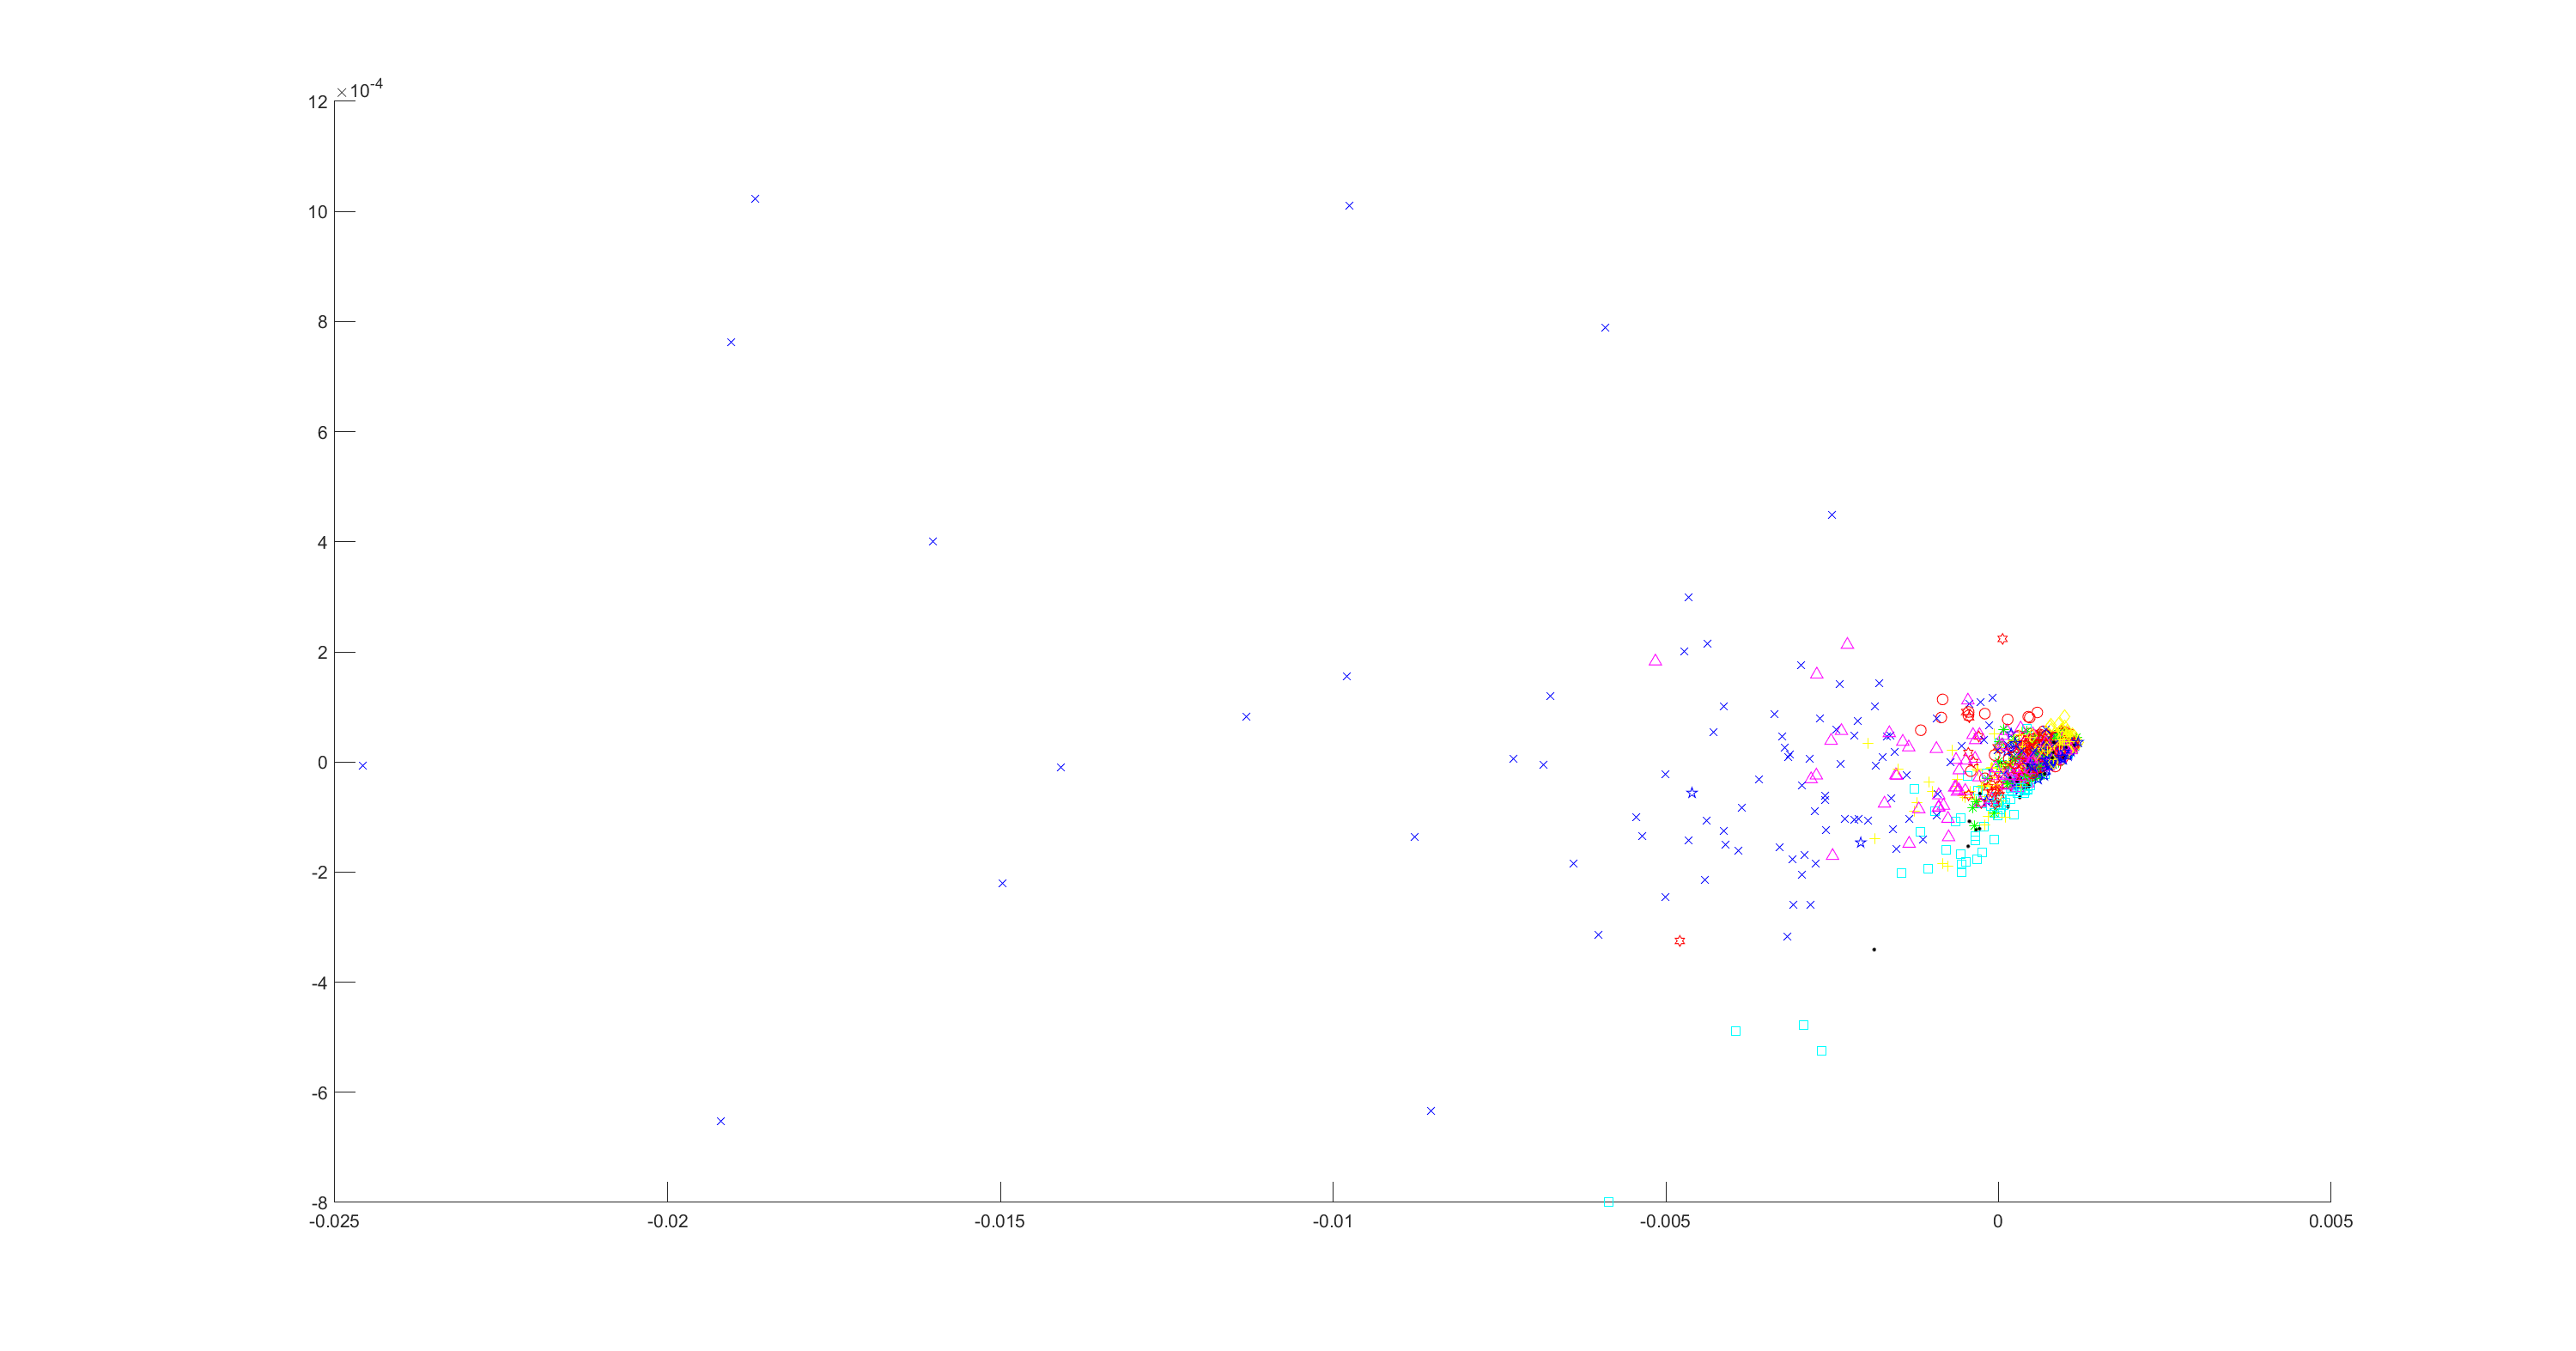
\includegraphics[width=1\textwidth]{images/patterns_pca.png}
\caption{ppatterns after PCA}
\label{fig:myimage}
\end{figure}

Even though we can only visualize data in 3D dimensions it is possible to have a notion of how is the data distributed in higher dimensions by analyzing its projection in lower, visualizable dimensions. In this case, we can see that after applying PCA to the dataset, the variance of the data is visibly predominant in one (of possibly many) directions. 

\begin{figure}[H]
\centering
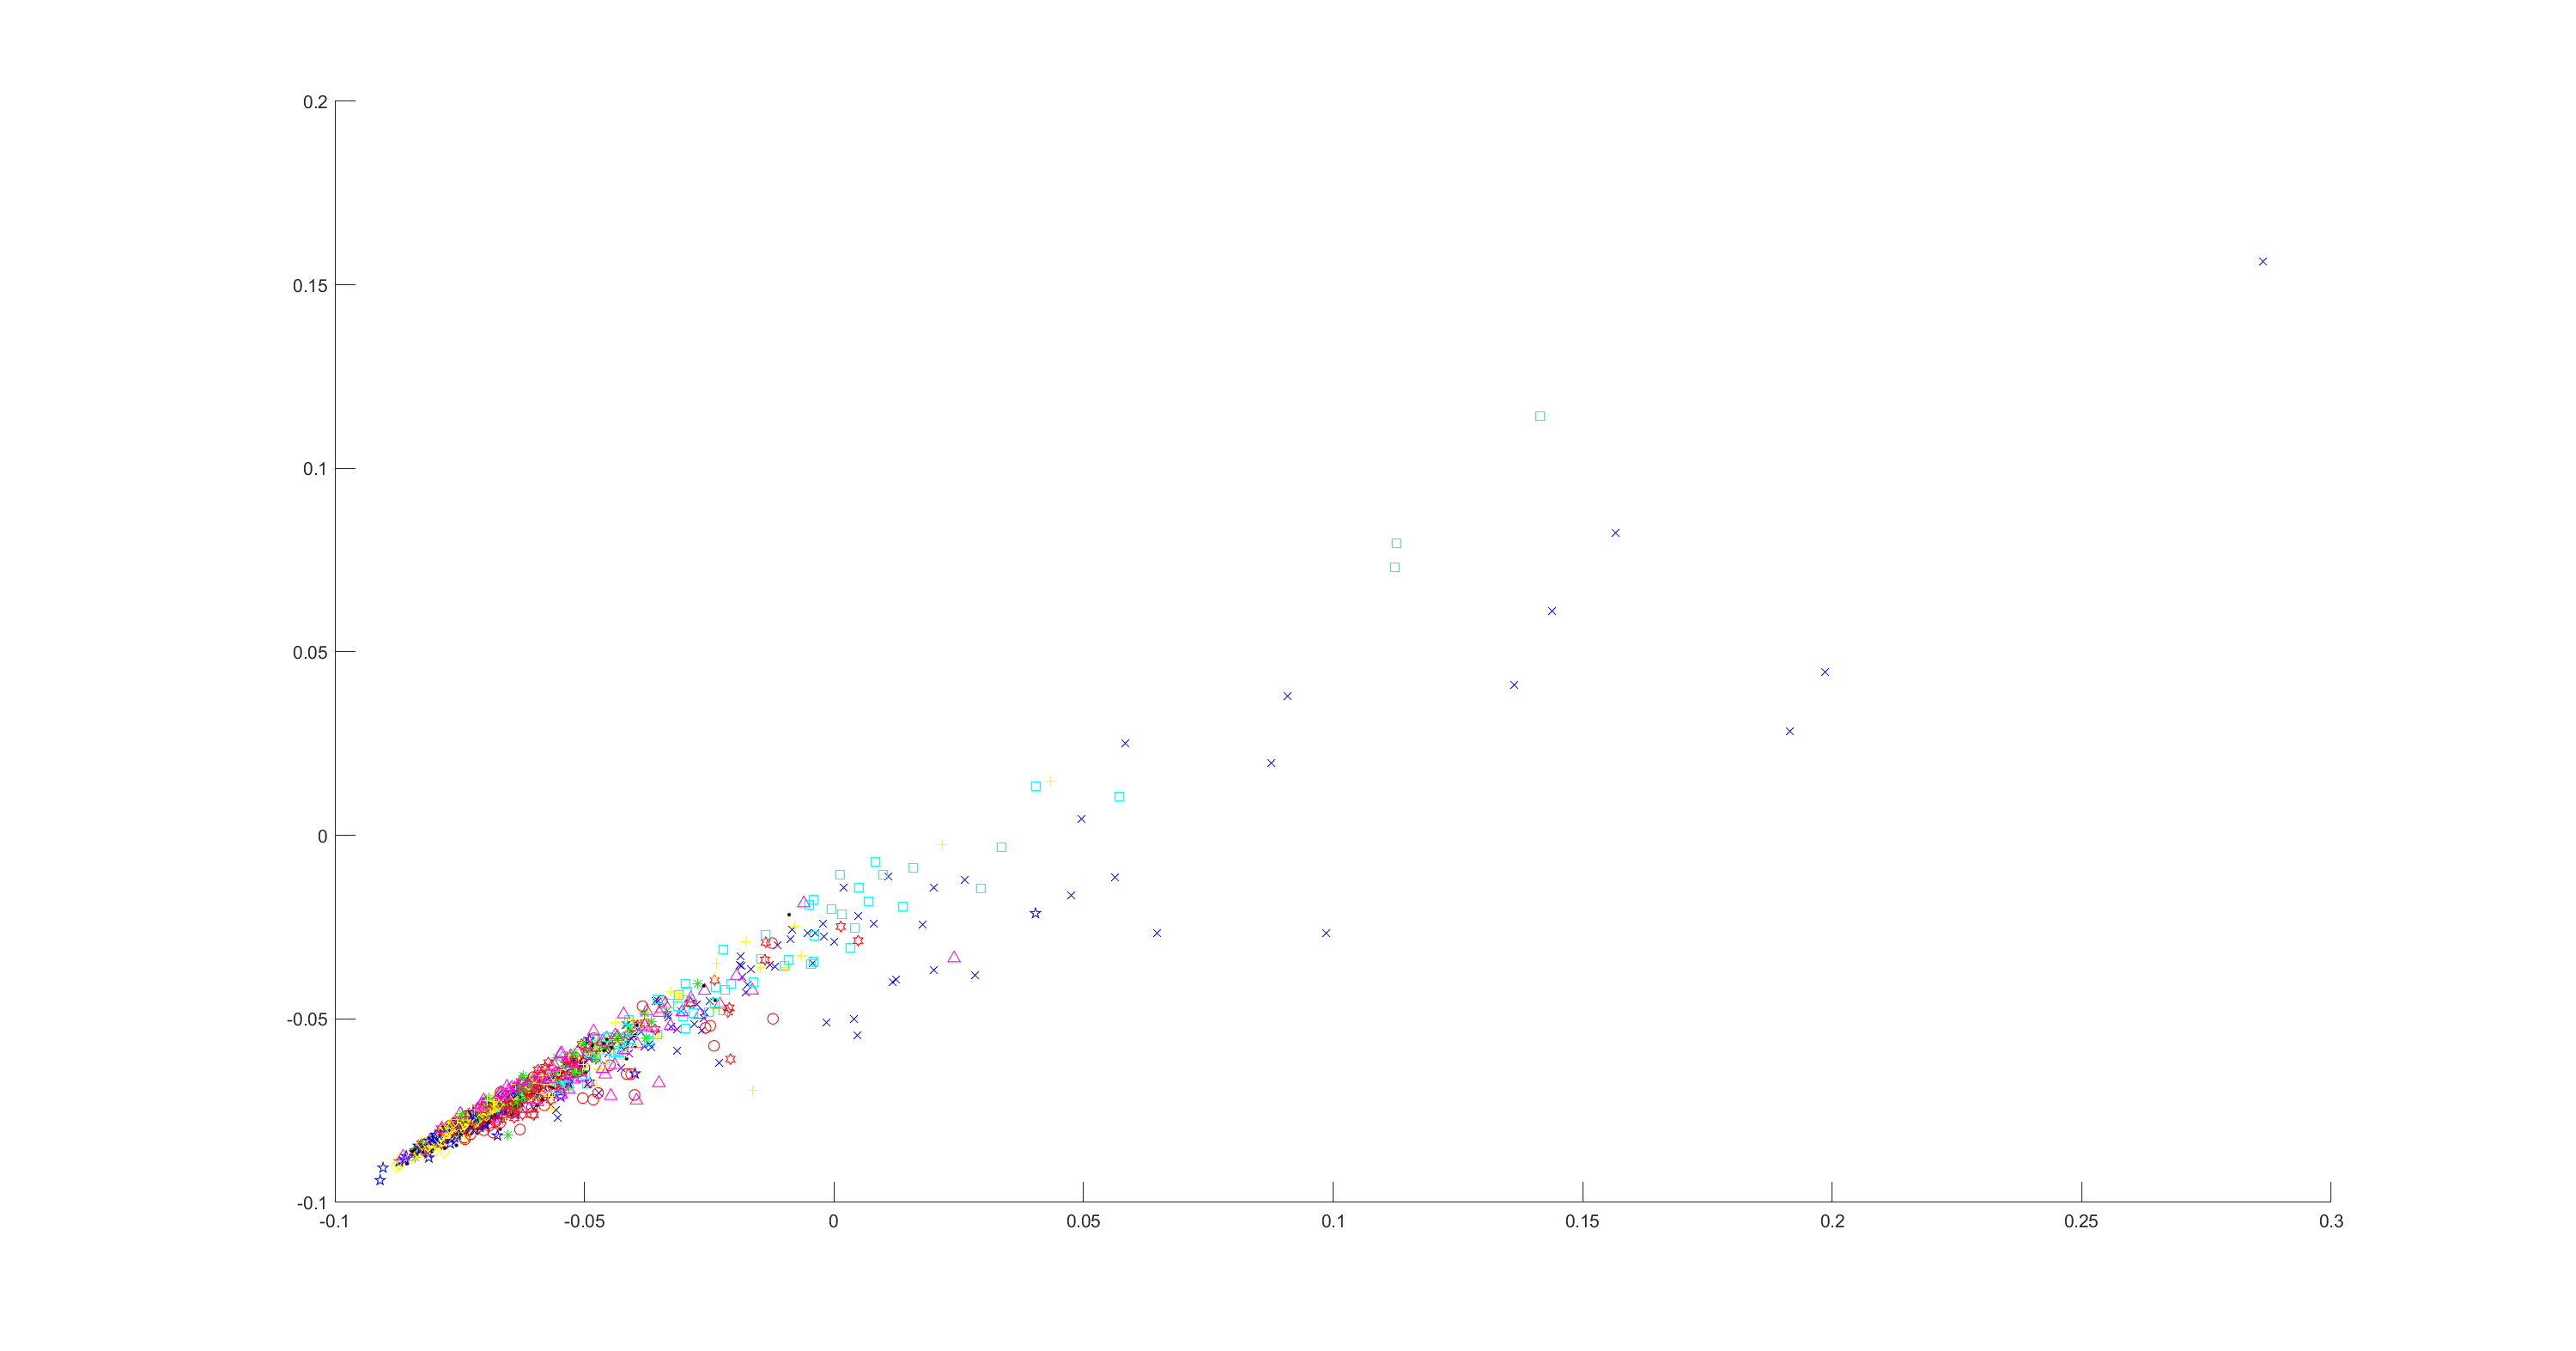
\includegraphics[width=1\textwidth]{images/patterns_pca_kw.png}
\caption{ppatterns after PCA + KW}
\label{fig:myimage}
\end{figure}

After applying Kruskal-Wallis to the data after PCA, it is possible to observe some emerging clusters, even though we are in visualizing the feature space projected in a lower dimensional space. This indicates that the dataset is becoming more linearly separable during the feature selection/reduction process. 

\begin{figure}[H]
\centering
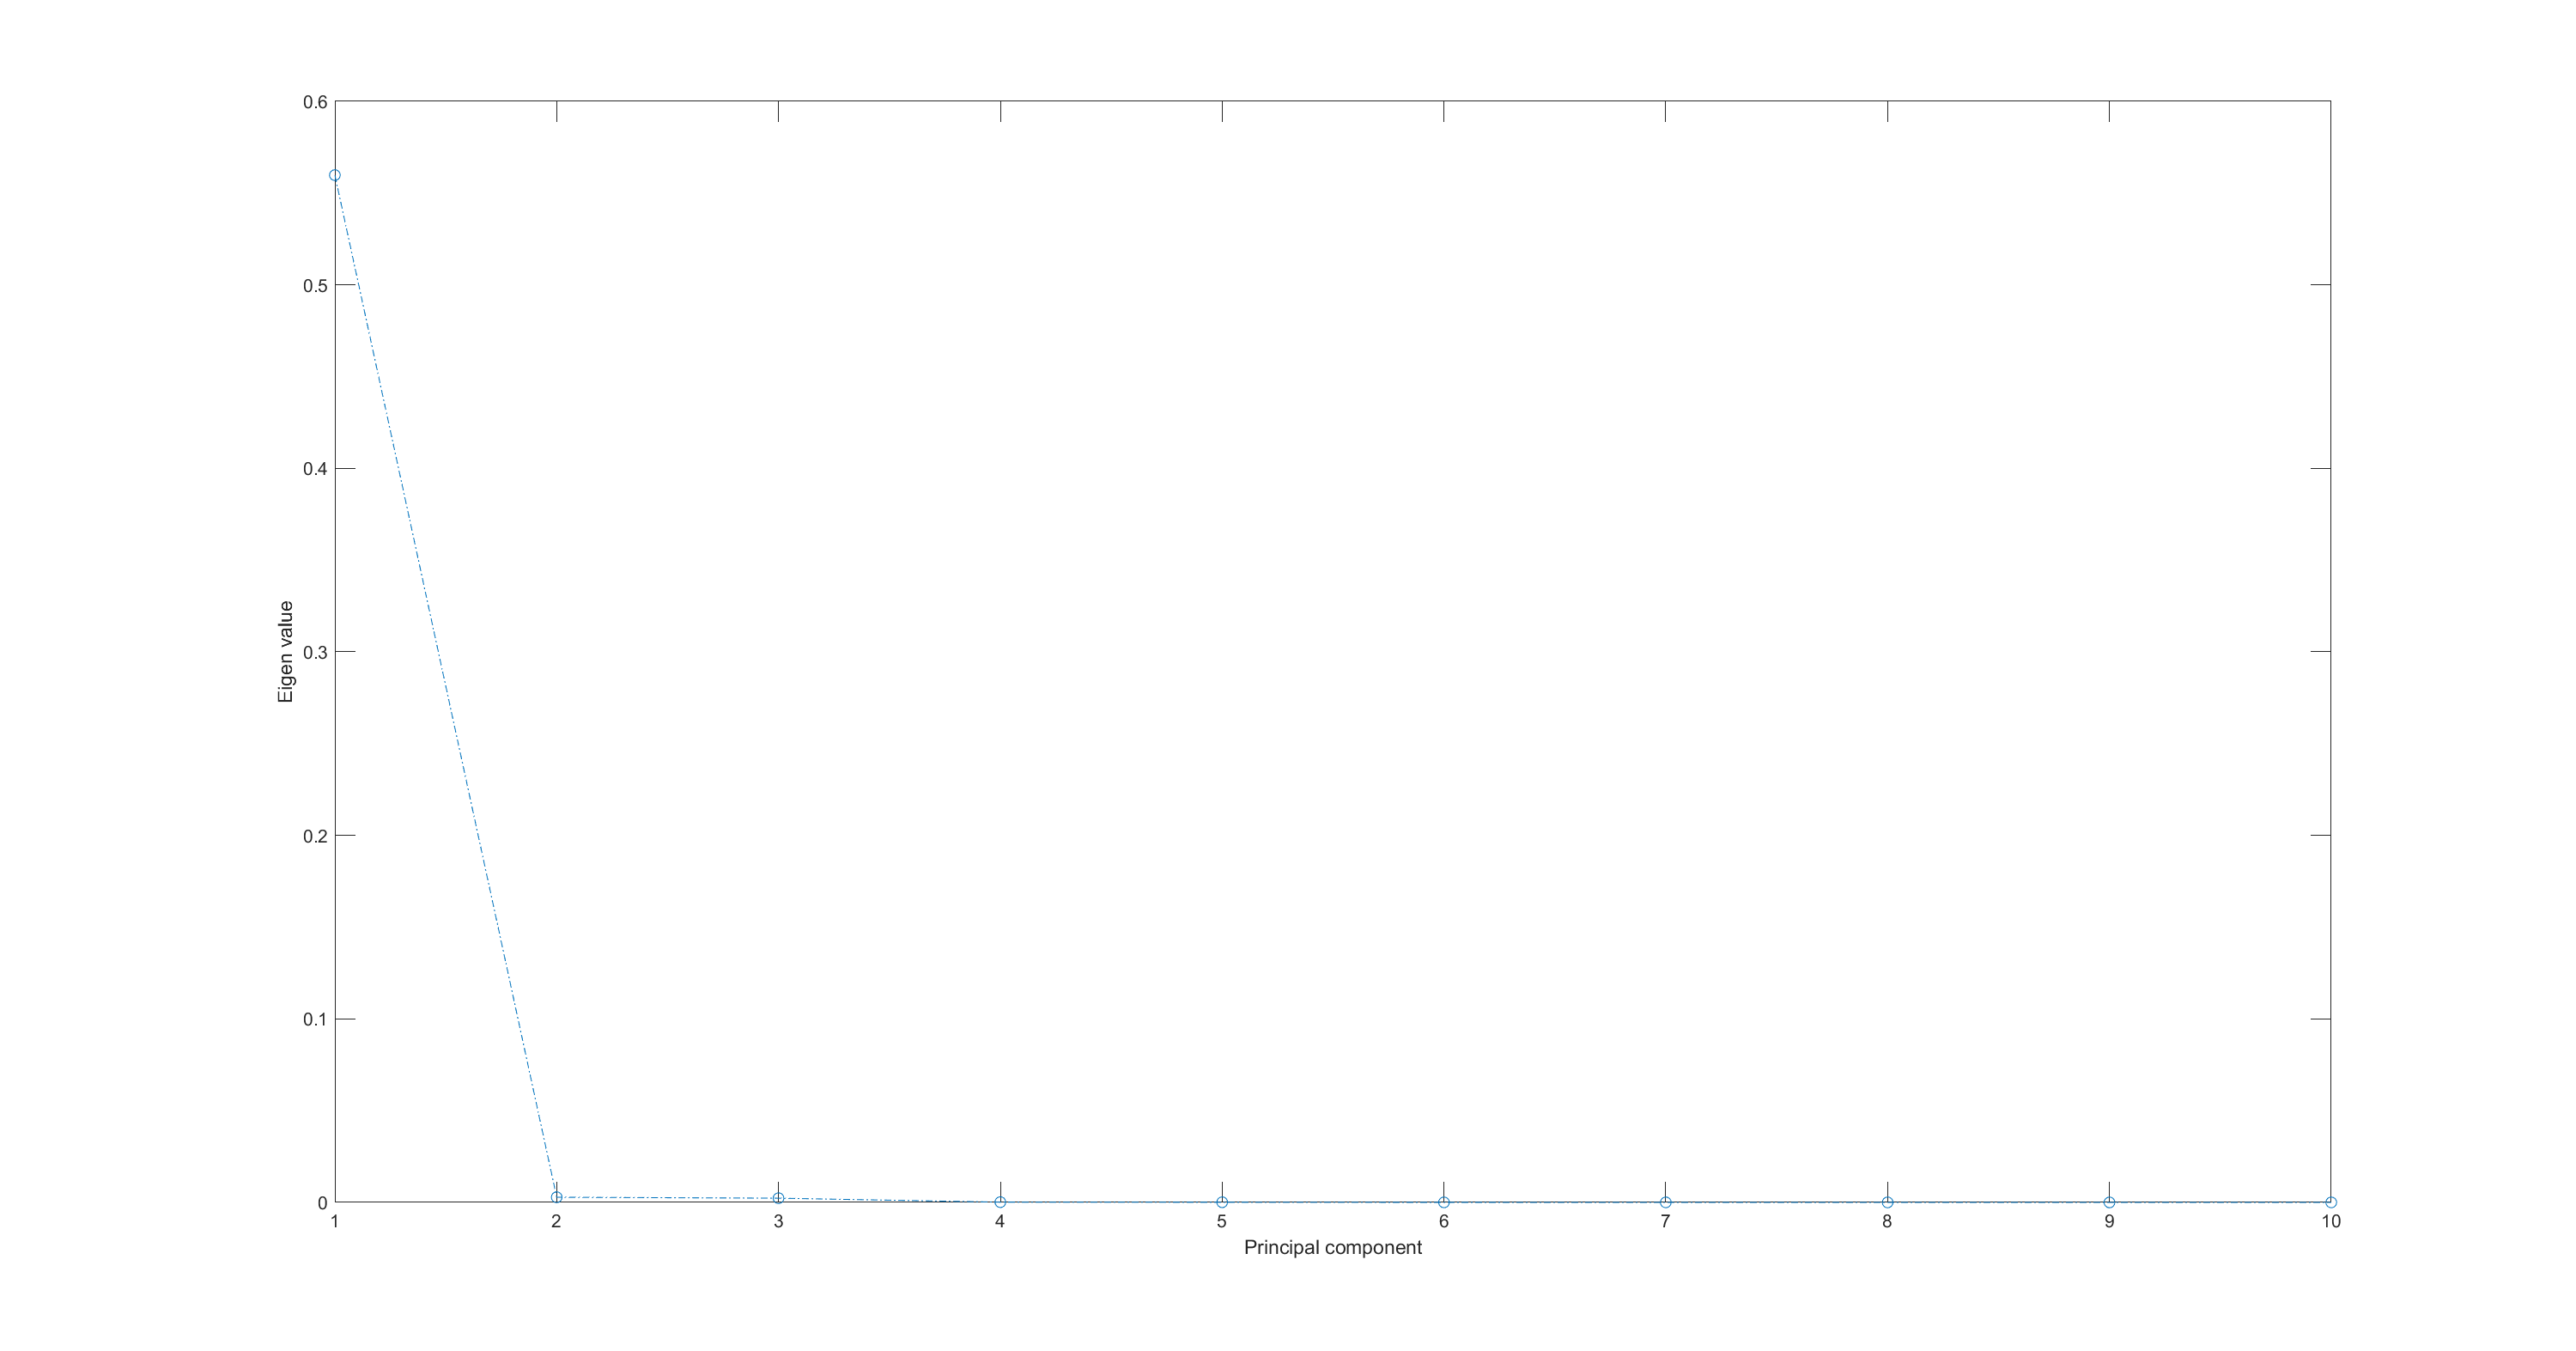
\includegraphics[width=1\textwidth]{images/pca_eigen_values_zscore.png}
\caption{PCA Eigen Values with Z-score normalization}
\label{fig:myimage}
\end{figure}

\begin{figure}[H]
\centering
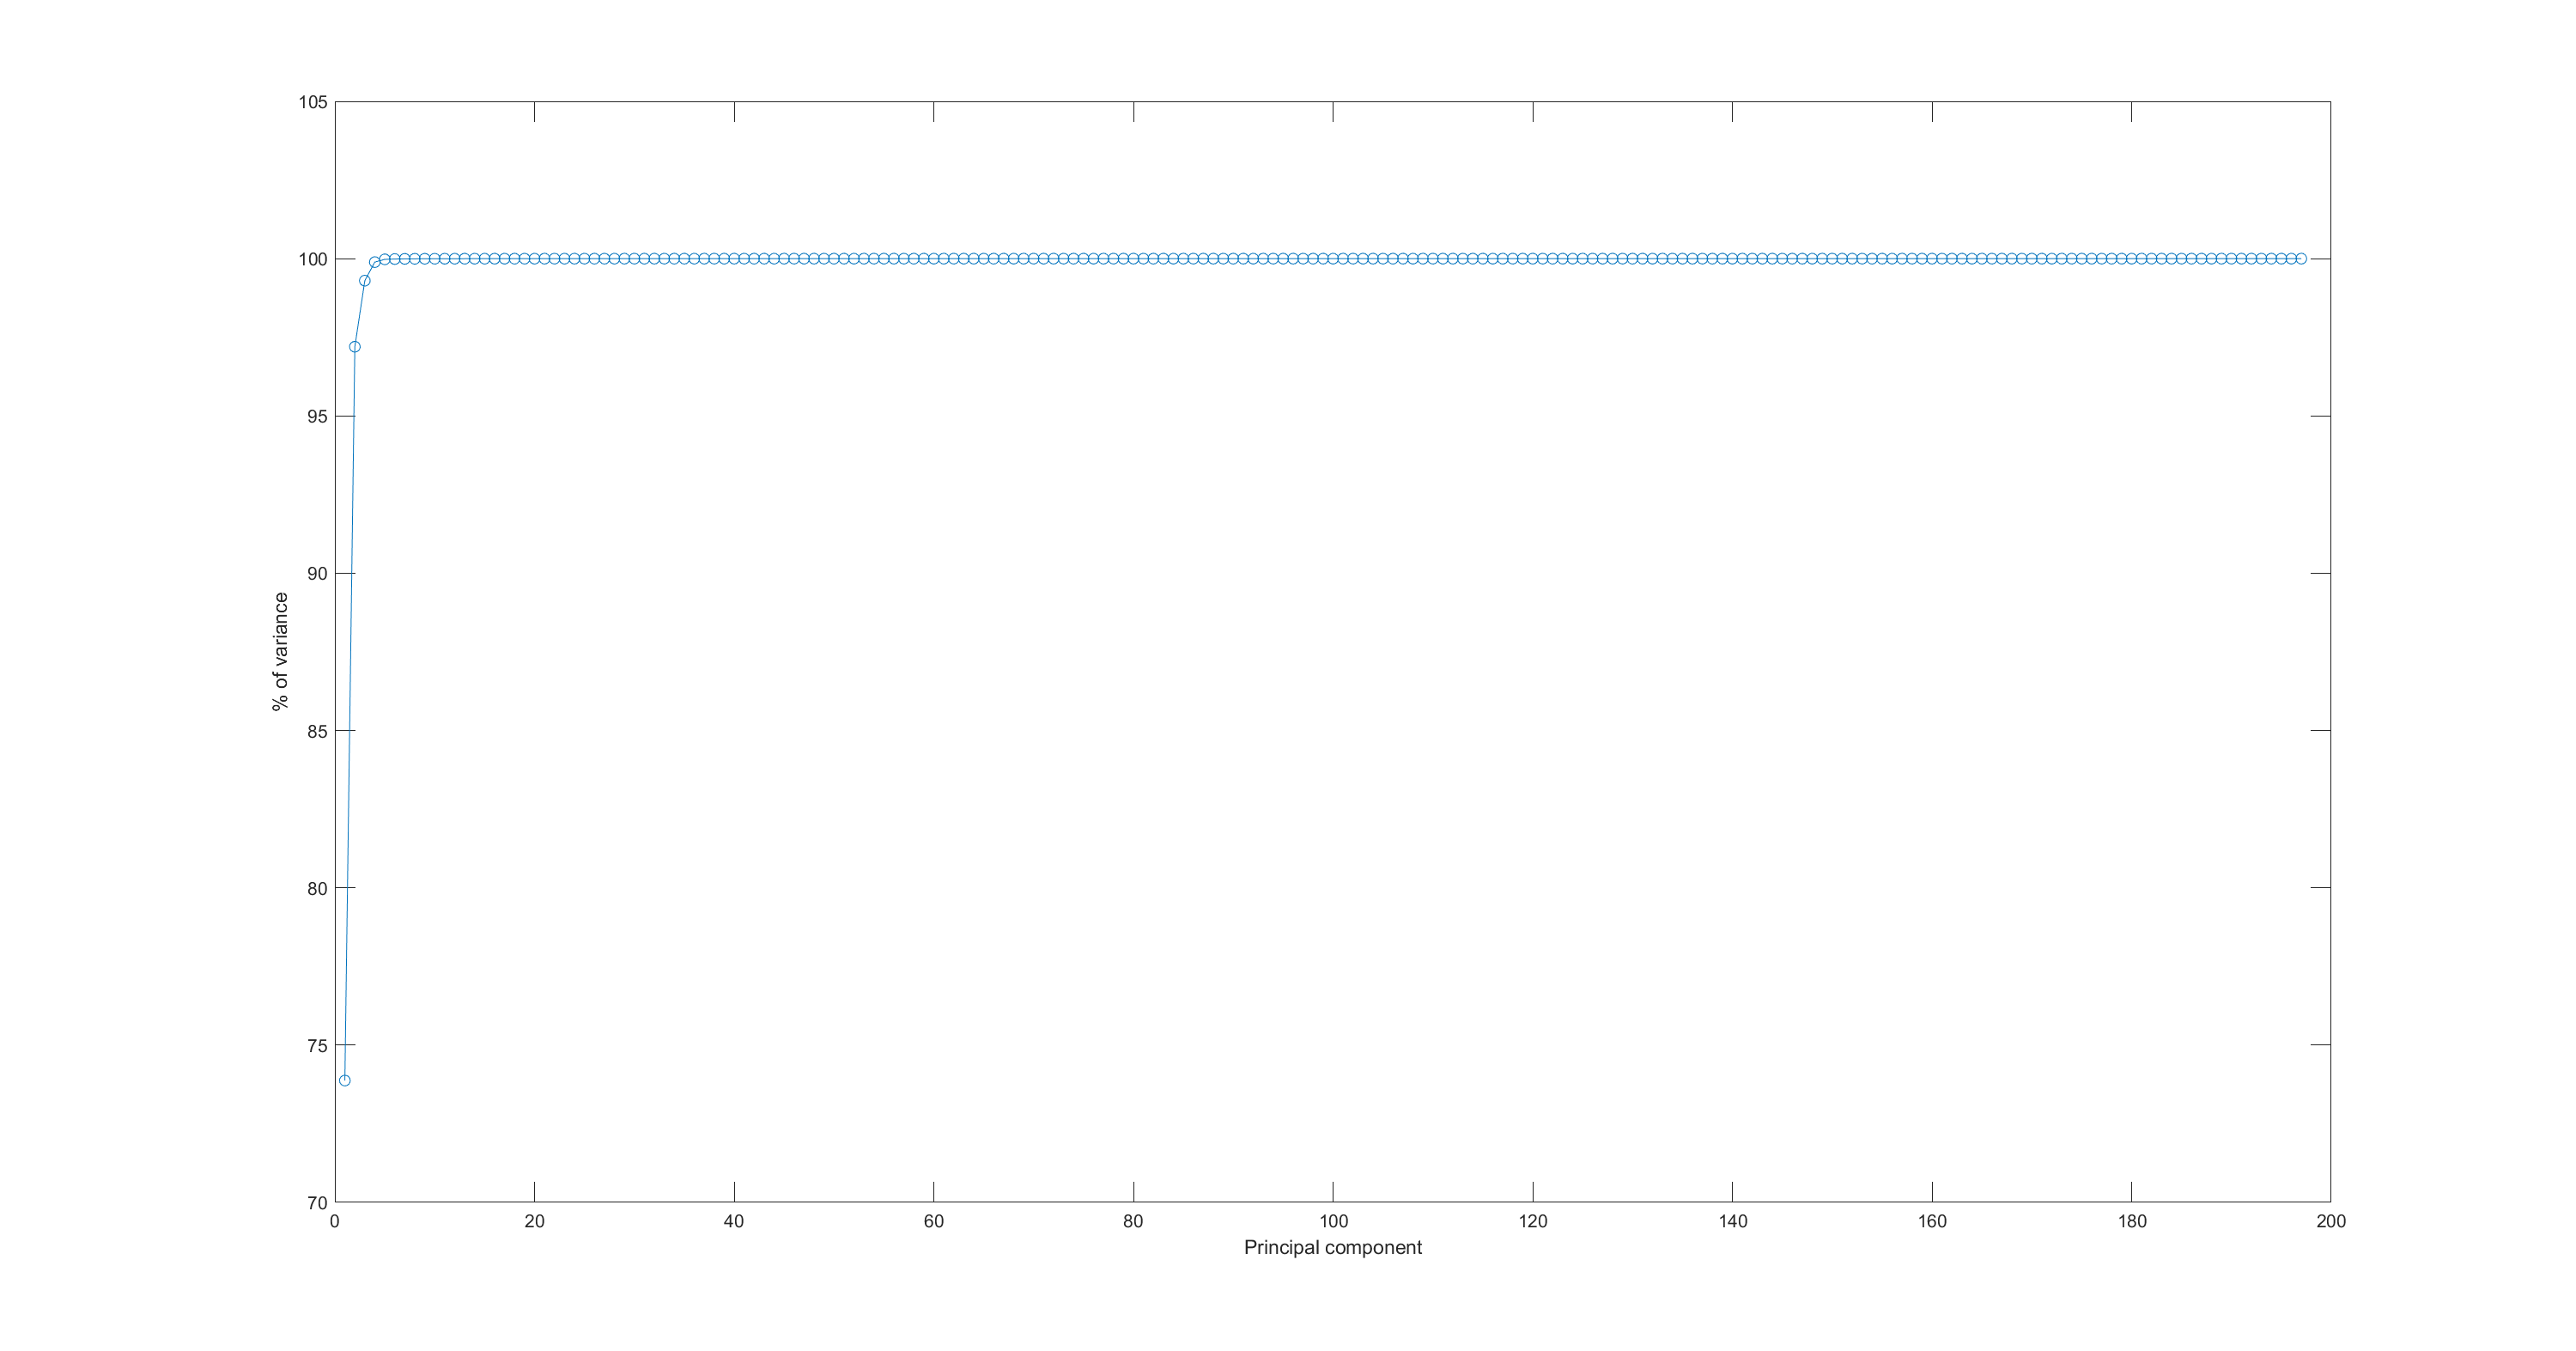
\includegraphics[width=1\textwidth]{images/pca_variance_zscore.png}
\caption{PCA variance with Z-score normalization}
\label{fig:myimage}
\end{figure}

After analyzing the graphs above, it is possible to deduce that there are only a handful of features that contribute to the overall variance of the dataset. Despite that fact, a more conservative attitude was taken when applying PCA to the GTZAN dataset, instead of simply taking the mentioned features. This is because, as mentioned before, PCA only captures the variance of each component and variance isn't the only measure of importance for a given feature.


\subsection{Kruskal Wallis}

Kruskal-Wallis is used to determine which features are most significant in differentiating between different classes in a dataset. The test ranks the features based on their ability to discriminate between classes, with higher-ranked features indicating a stronger correlation between the feature and class label. Overall, Kruskal-Wallis is a useful tool in feature selection as it provides a statistical measure of the importance of each feature in differentiating between classes, allowing researchers to focus on the most significant features in their analysis.

\begin{figure}[H]
\centering
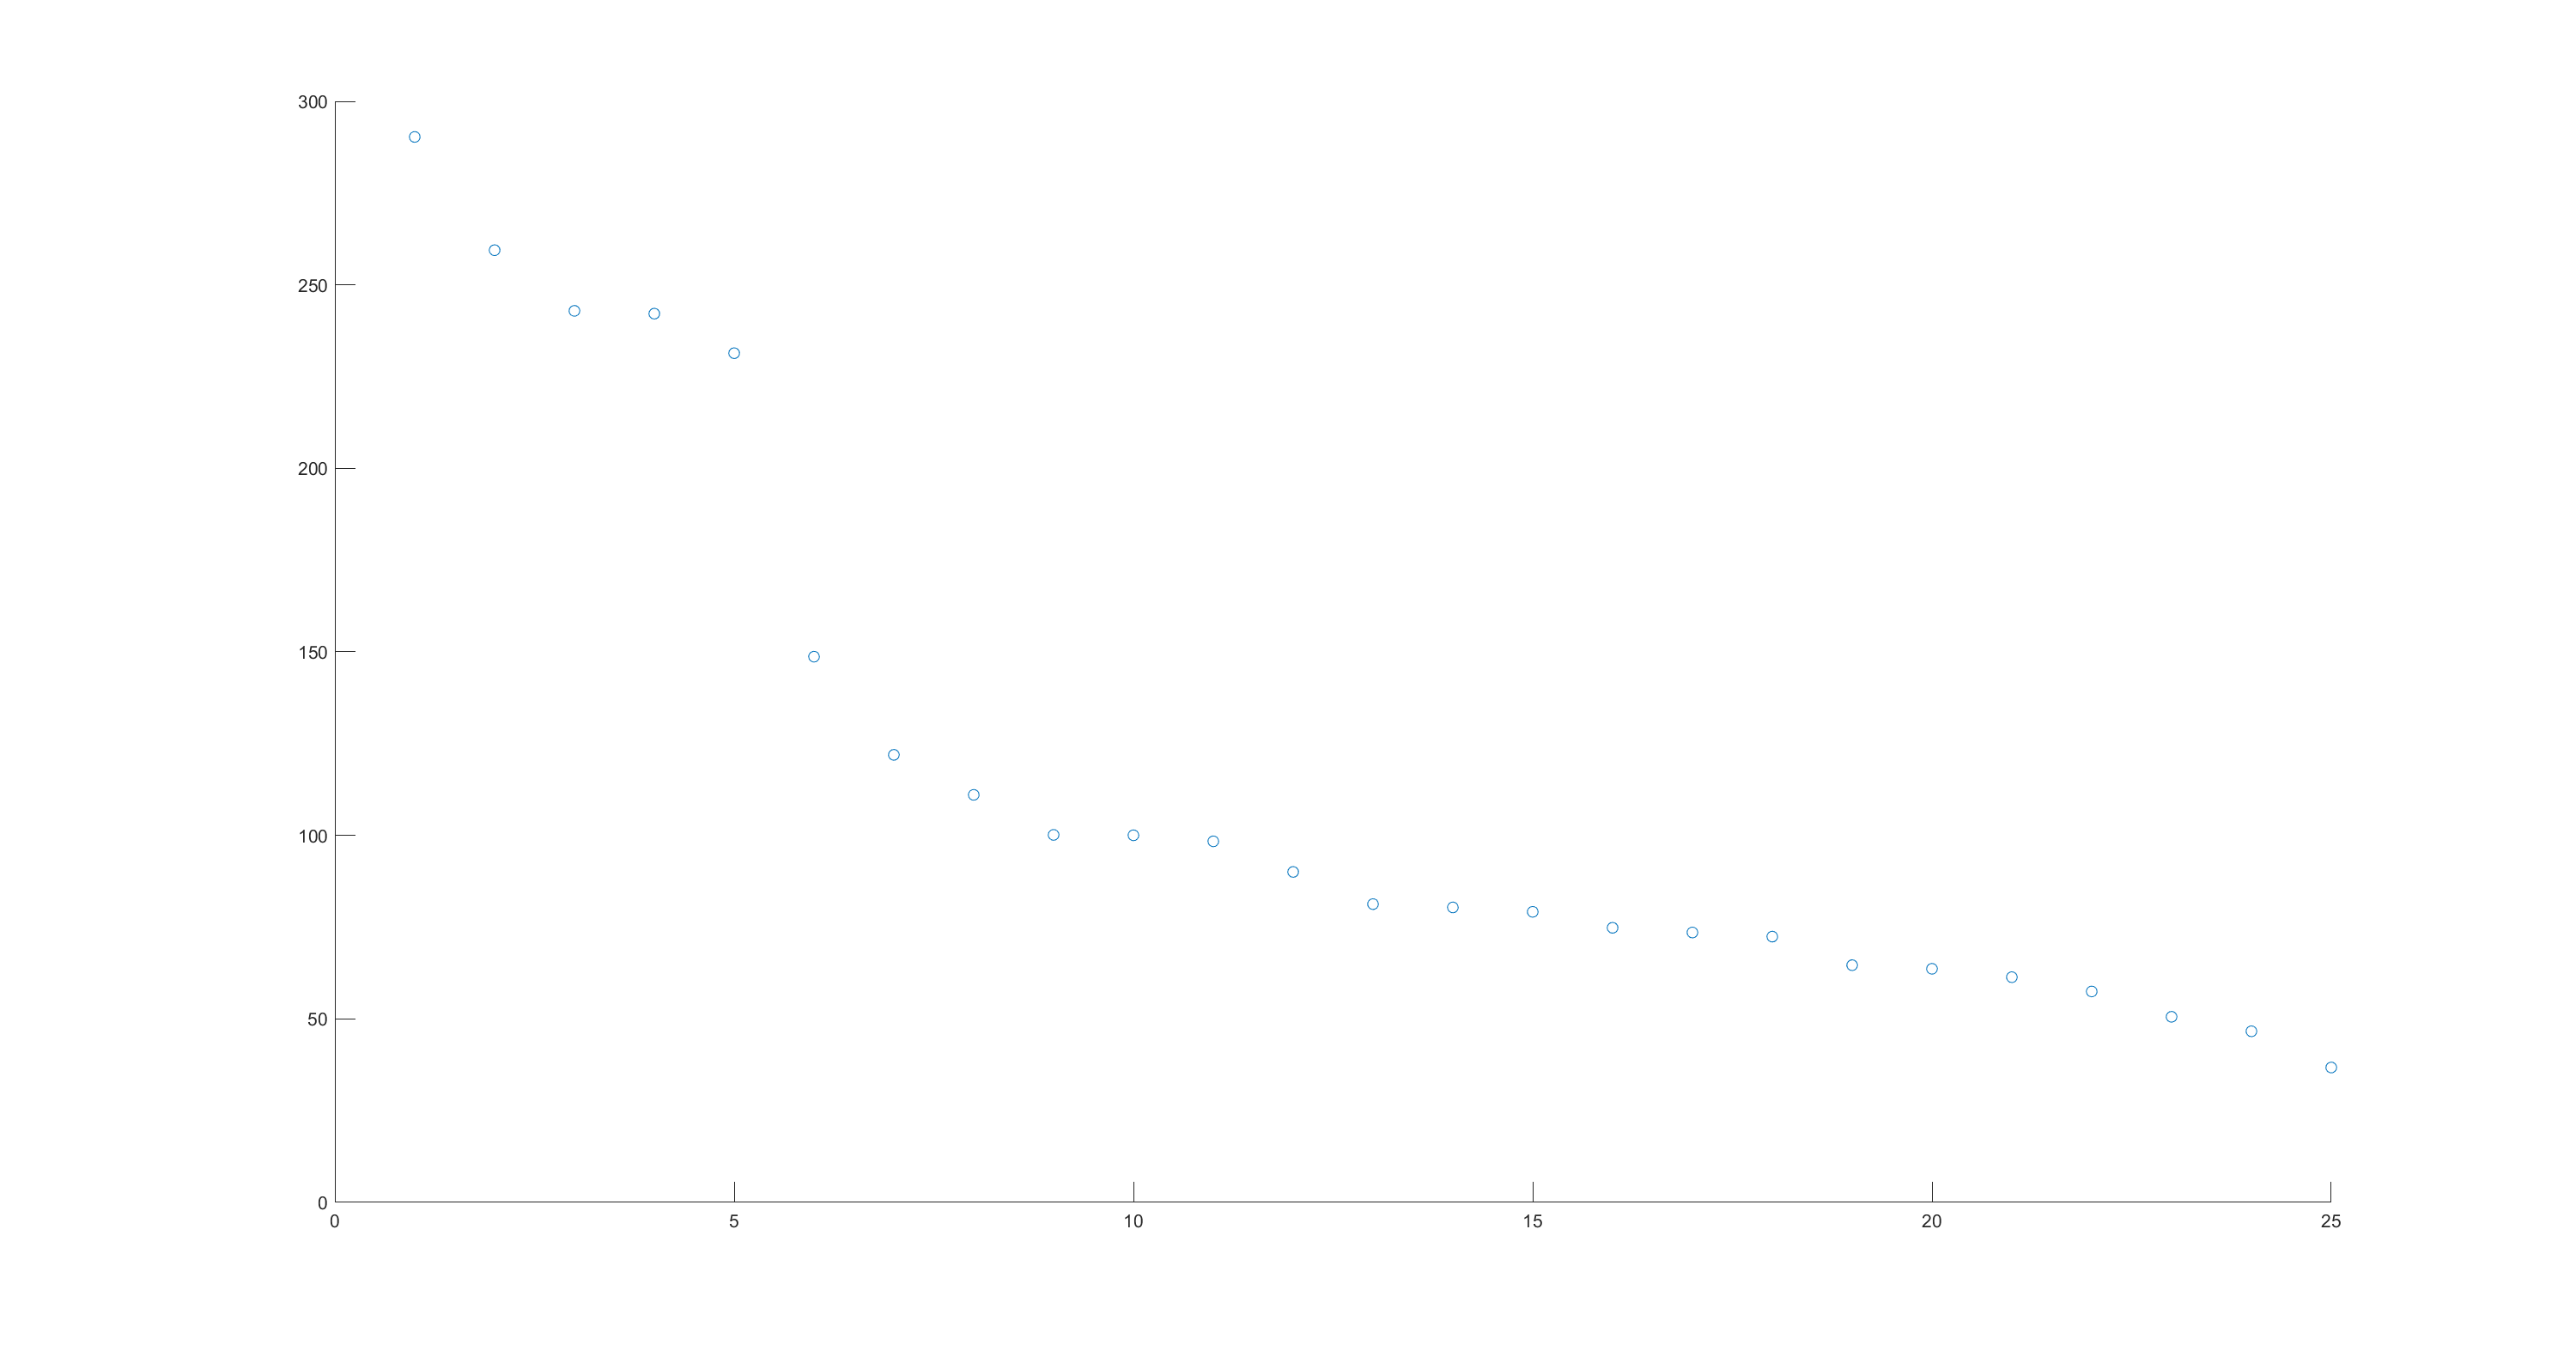
\includegraphics[width=1\textwidth]{images/scatter_h_kw.png}
\caption{KW scatter ranking}
\label{fig:myimage}
\end{figure}

\subsection{Correlation}

A correlation matrix is a table that displays the correlation coefficients between pairs of variables. 

In a correlation matrix, each row and column represents a variable, and the cells in the matrix show the correlation coefficients between each pair of variables. The diagonal cells always have a correlation coefficient of 1.0 because they represent the correlation between a variable and itself.

Correlation matrices are useful for identifying patterns and relationships between variables in a dataset. They can help to identify variables that are strongly related to each other, which can be useful for developing predictive models or understanding complex systems.

In the context of feature selection or reduction, correlation refers to the degree to which two or more variables are linearly related. When there is a high correlation between two variables, they provide redundant information to a machine learning model. In other words, they provide similar information, and using both variables does not significantly improve the performance of the model.

When performing feature selection or reduction, the goal is to select a subset of features that are most relevant for predicting the target variable. Having correlated features in the dataset can lead to several issues in this process:

\textbf{Redundant features}: Correlated features can provide redundant information to the model, which can increase the complexity of the model and slow down training time. This can also lead to overfitting, where the model performs well on the training data but poorly on new, unseen data.

\textbf{Unstable model}: When two or more features are highly correlated, small changes in one feature can lead to significant changes in the other feature. This can make the model unstable and difficult to interpret.

\textbf{Decreased model accuracy}: Correlated features can also decrease the accuracy of the model, as they can introduce bias and noise into the model. This can lead to inaccurate predictions and reduced performance.

Therefore, in feature selection or reduction, the existence of correlation is generally undesired as it can negatively impact the performance and stability of the model. To mitigate this issue, techniques such as correlation analysis or principal component analysis (PCA) can be used to identify and remove correlated features from the dataset.

To gain insight into the interdependence of the variables, we constructed a correlation matrix for every normalization and feature reduction method, and in all combinations, the results showed us that the variables had almost no correlation with each other. Below there is an example of two of the correlation matrices obtained:

\begin{figure}[H]
\centering
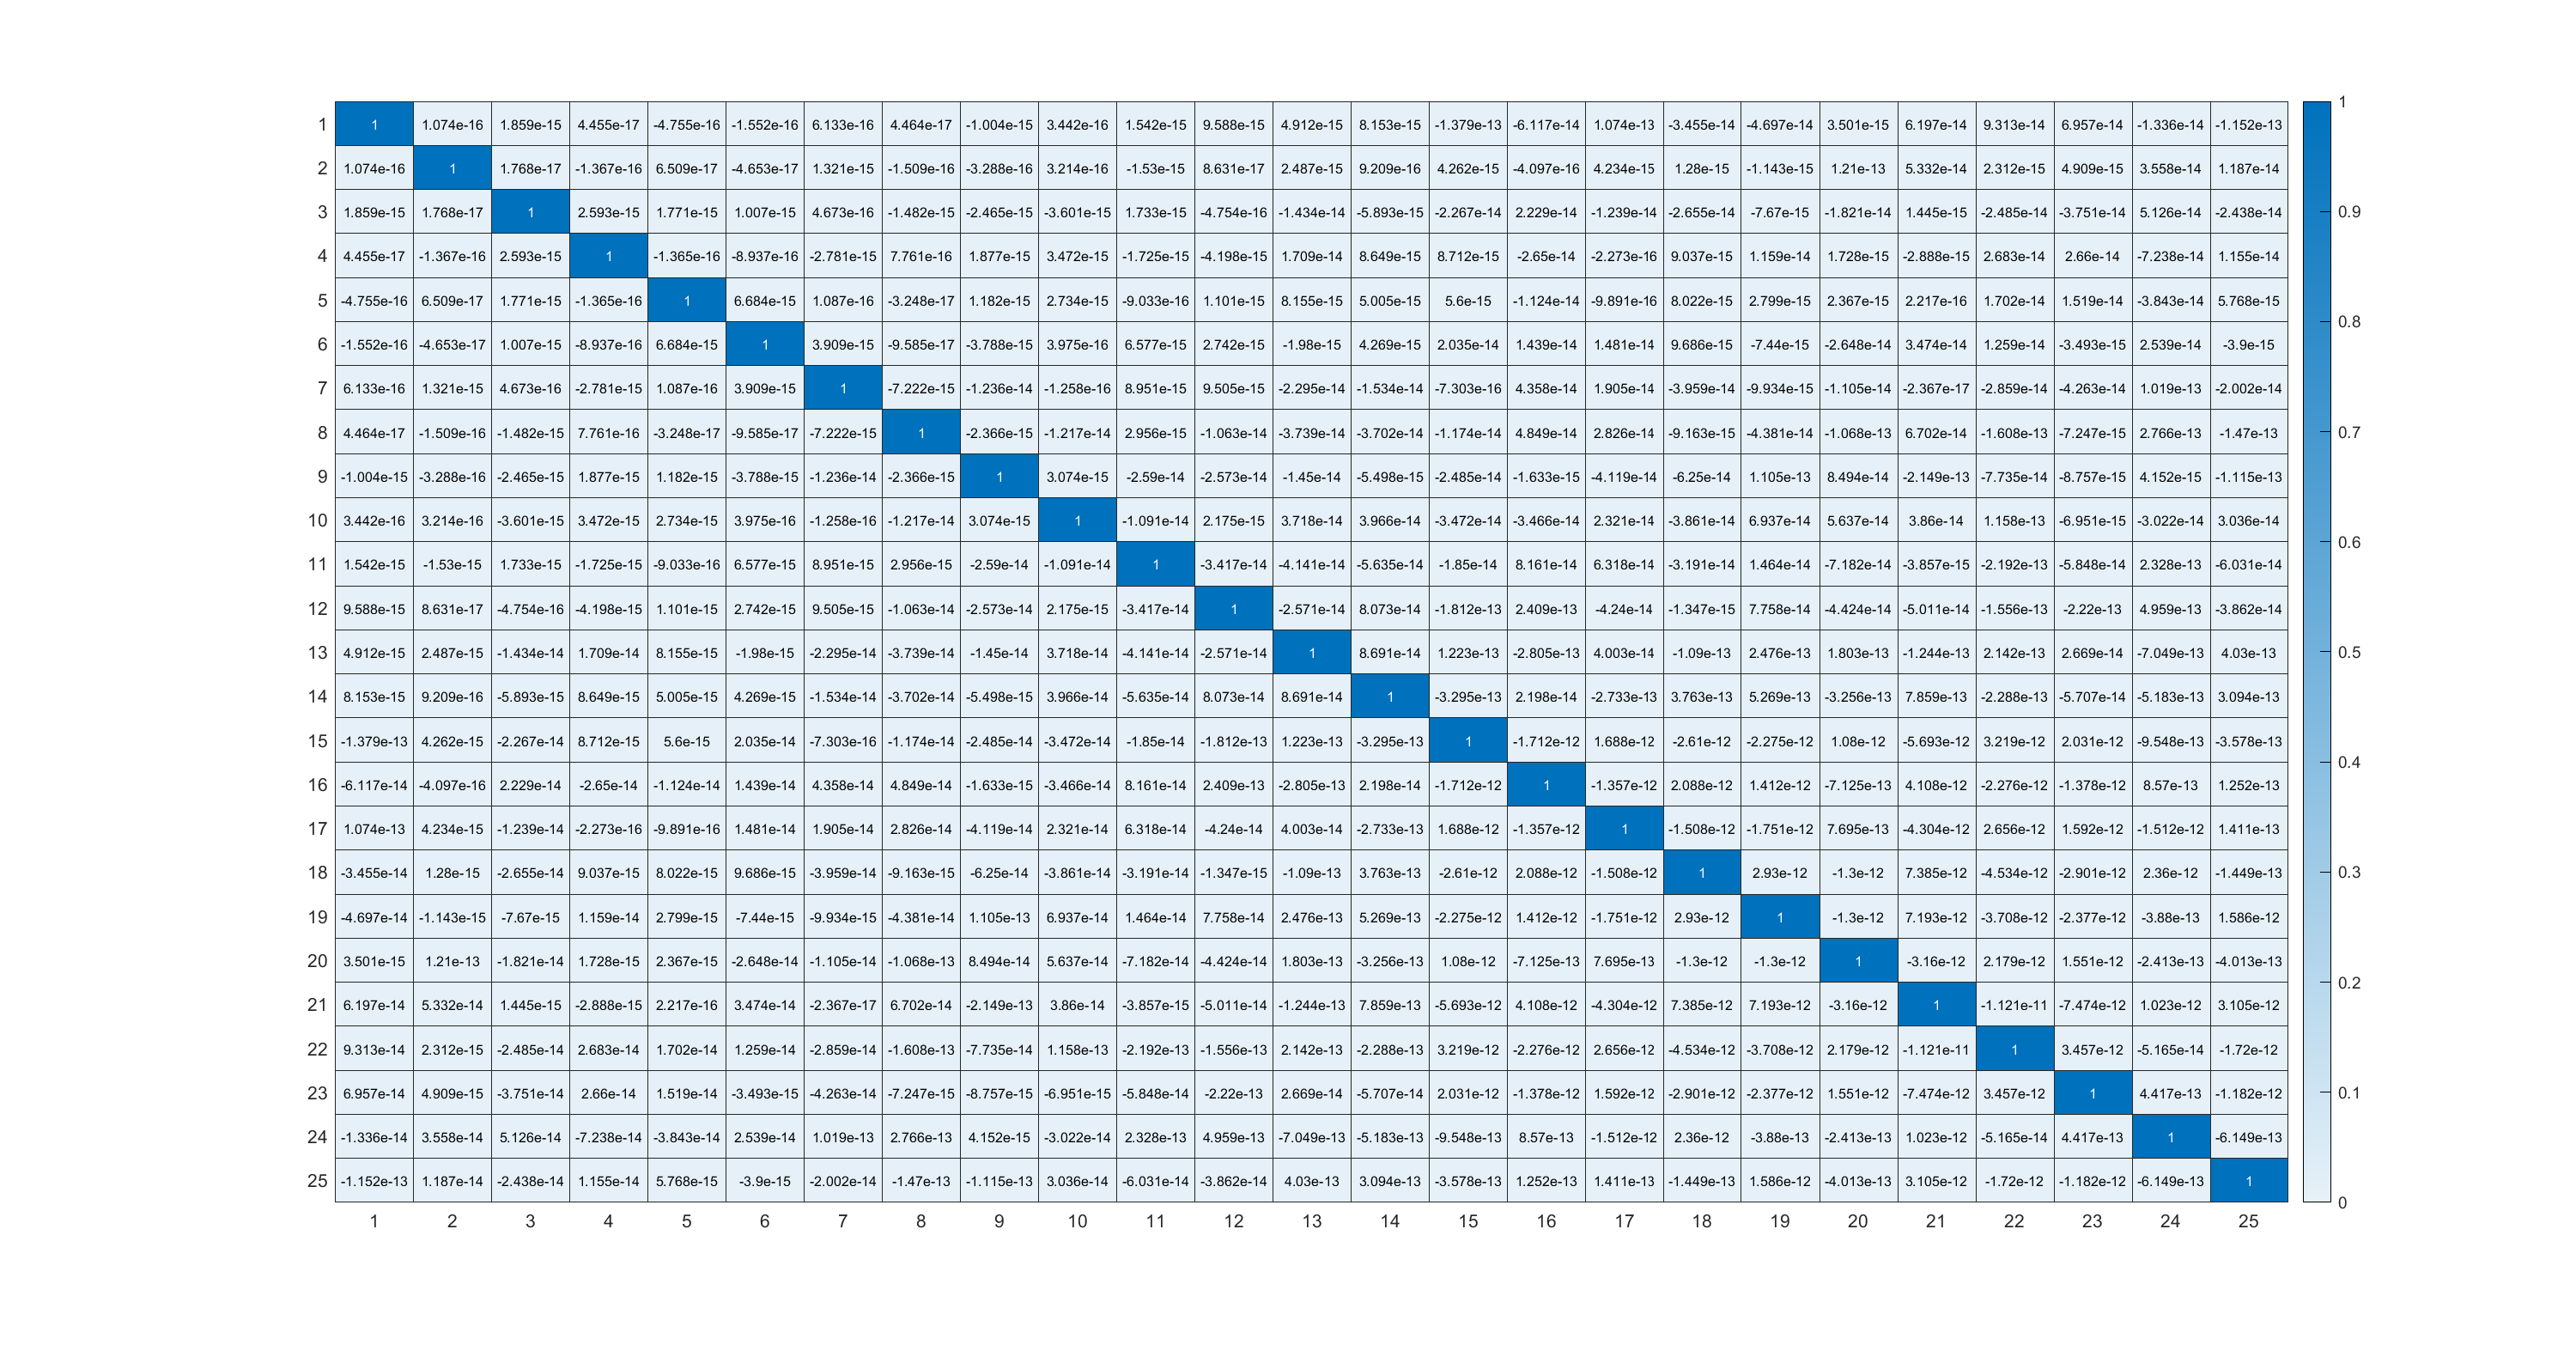
\includegraphics[width=1\textwidth]{images/corr_matrix_pca_zscore.png}
\caption{Correlation with "zscore" normalization after PCA }
\label{fig:myimage}
\end{figure}

\begin{figure}[H]
\centering
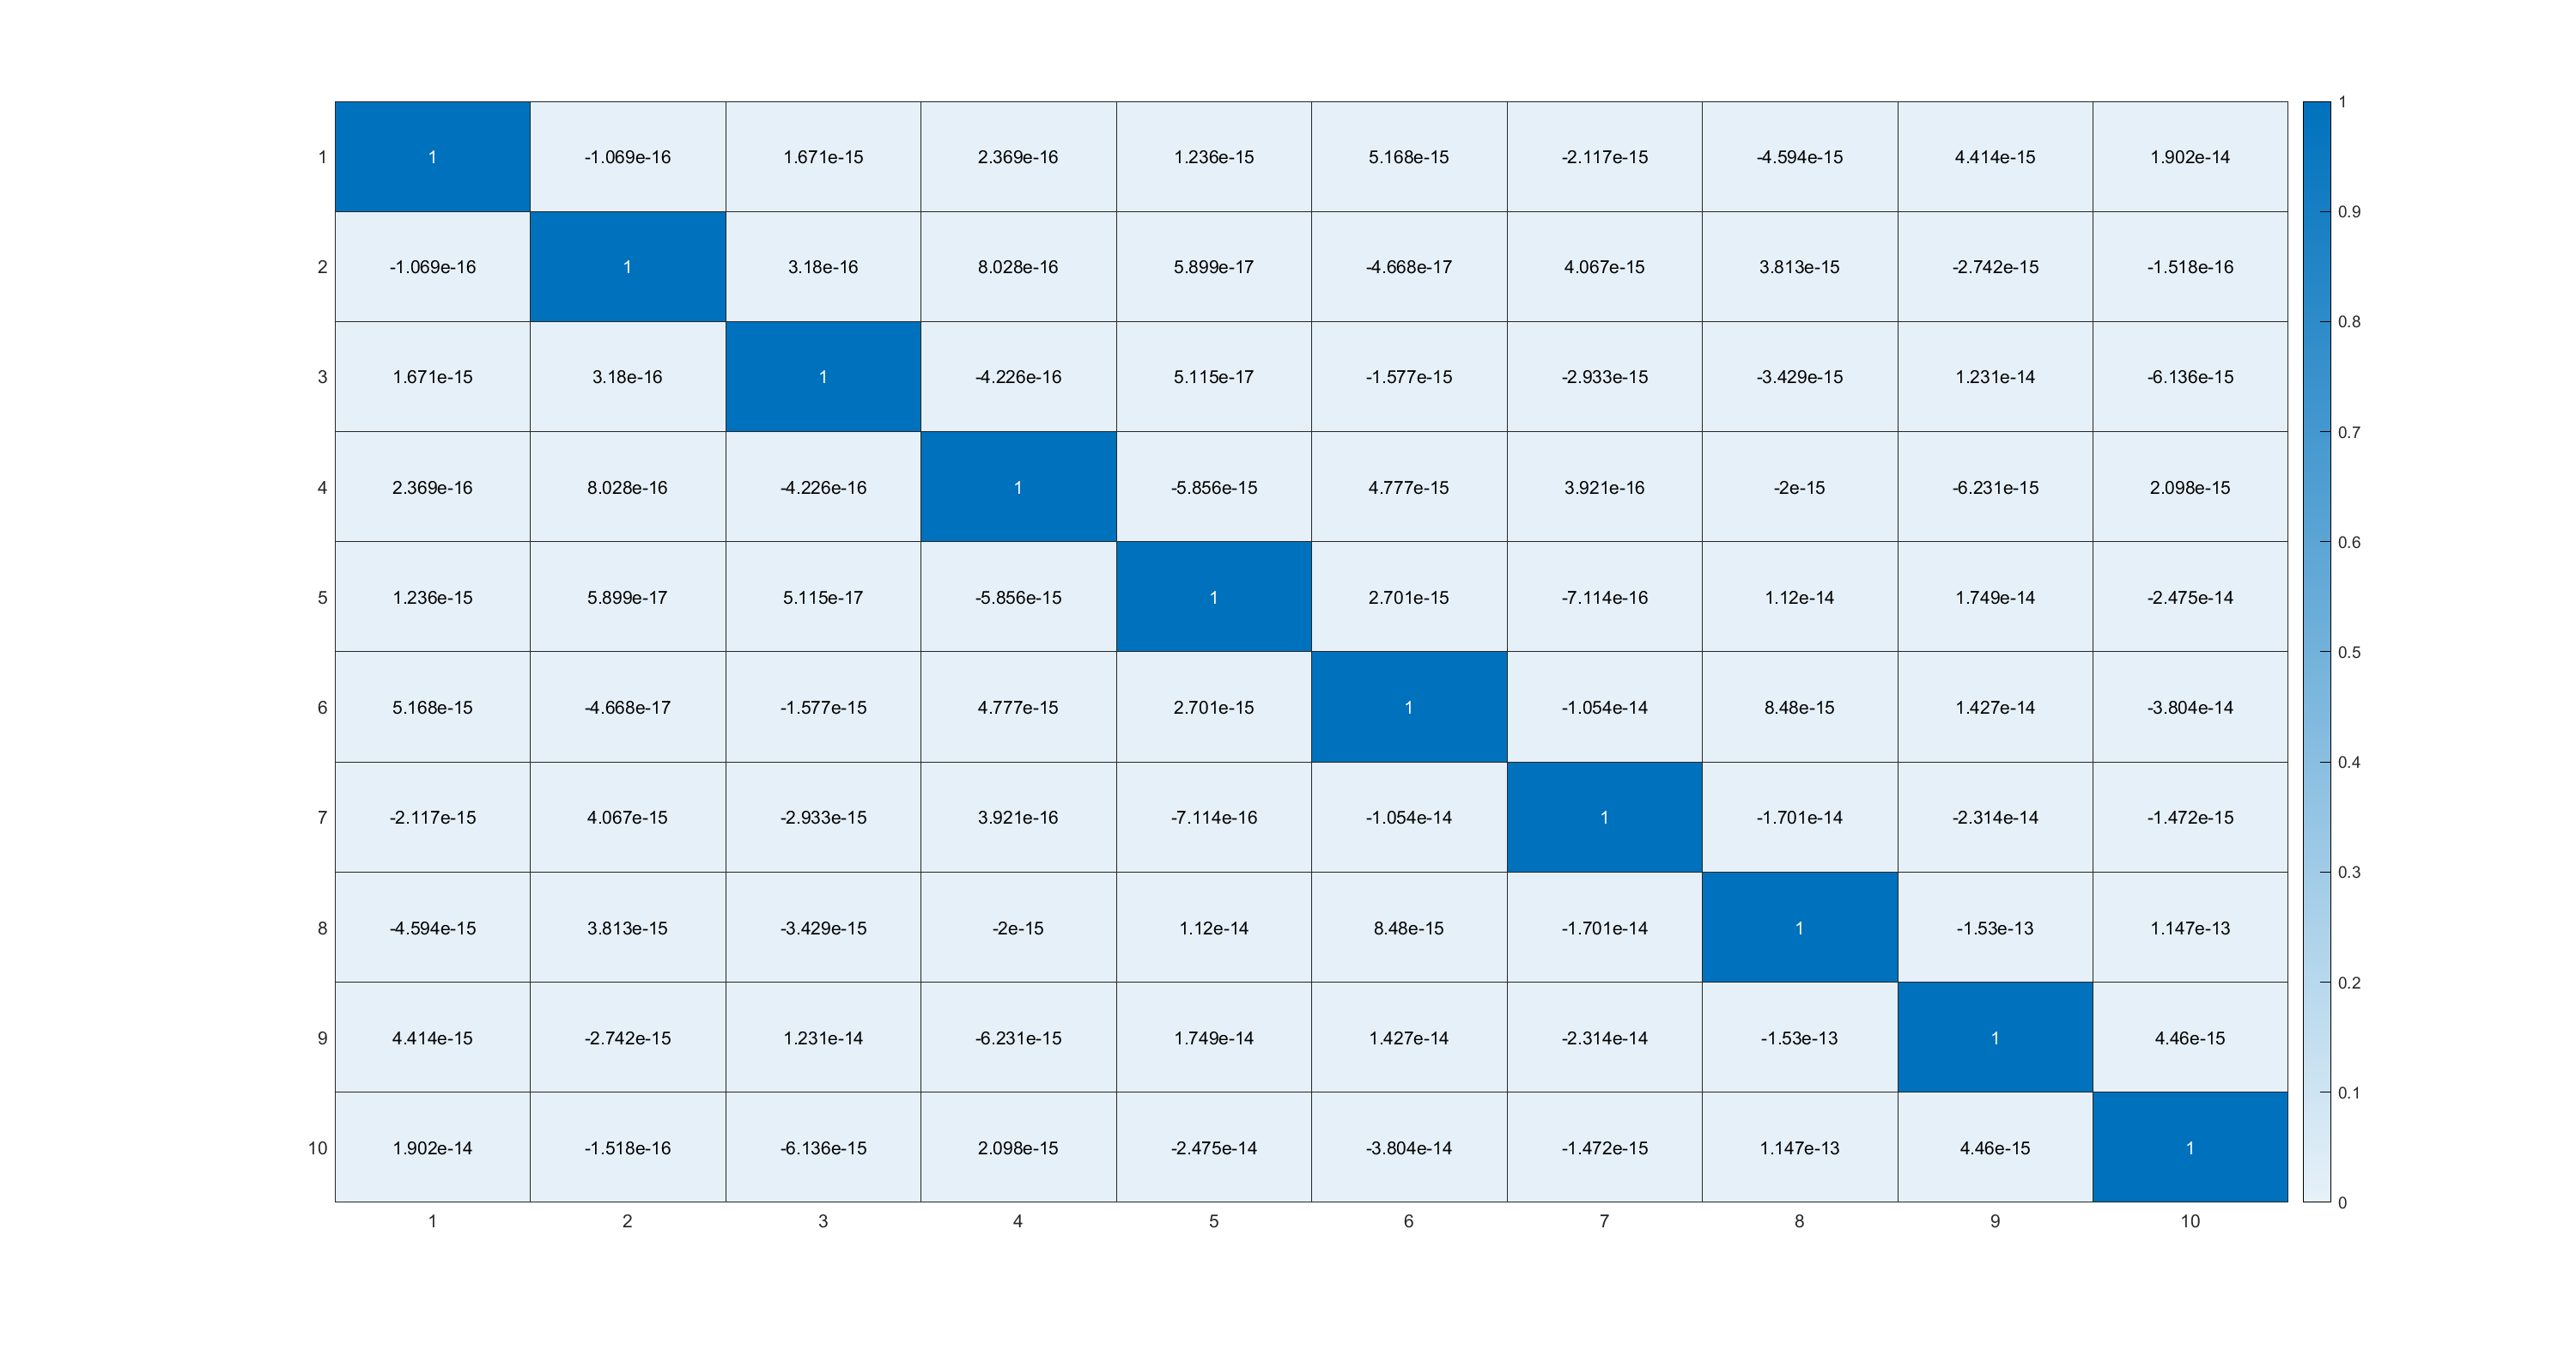
\includegraphics[width=1\textwidth]{images/corr_matrix_zscore.png}
\caption{Correlation with "zscore" normalization after PCA and KW }
\label{fig:myimage}
\end{figure}

\subsection{Random Forest}

A random forest is an ensemble learning method that constructs a multitude of decision trees at training time and outputs the class that is the mode of the classes (classification) or mean prediction (regression) of the individual trees. In the context of our project on music genre recognition, we can use a random forest to identify the most informative features for predicting the genre of a song based on its audio features.

Mathematically:
Let $X$ be a set of input audio features and $Y$ be the target variable representing the genre of a song. Random Forests construct $T$ decision trees, where each tree $t$ is built using a random subset of $m$ features from $X$. The predicted output of the Random Forest is the mode of the predicted outputs of the individual decision trees. 

In the context of our project on music genre recognition, we are interested in identifying the most informative audio features for predicting the genre of a song. Random Forests is a powerful method for feature reduction/selection because they can identify and prioritize the most informative features in the data. By constructing multiple decision trees and randomly selecting subsets of features, Random Forests can identify the features that are consistently important across the trees. This is reflected in the feature importance scores that are generated by the algorithm. Features with higher importance scores are more likely to be selected by the algorithm and can be used for feature reduction/selection.

Additionally, Random Forests can handle data with a large number of features and can capture nonlinear relationships between the features and the target variable. In the context of music genre recognition, this is important because there are likely to be complex relationships between the audio features and the genre of a song. By using a Random Forest to identify the most informative features, we can improve the accuracy of our music genre recognition model.

\begin{figure}[H]
\centering
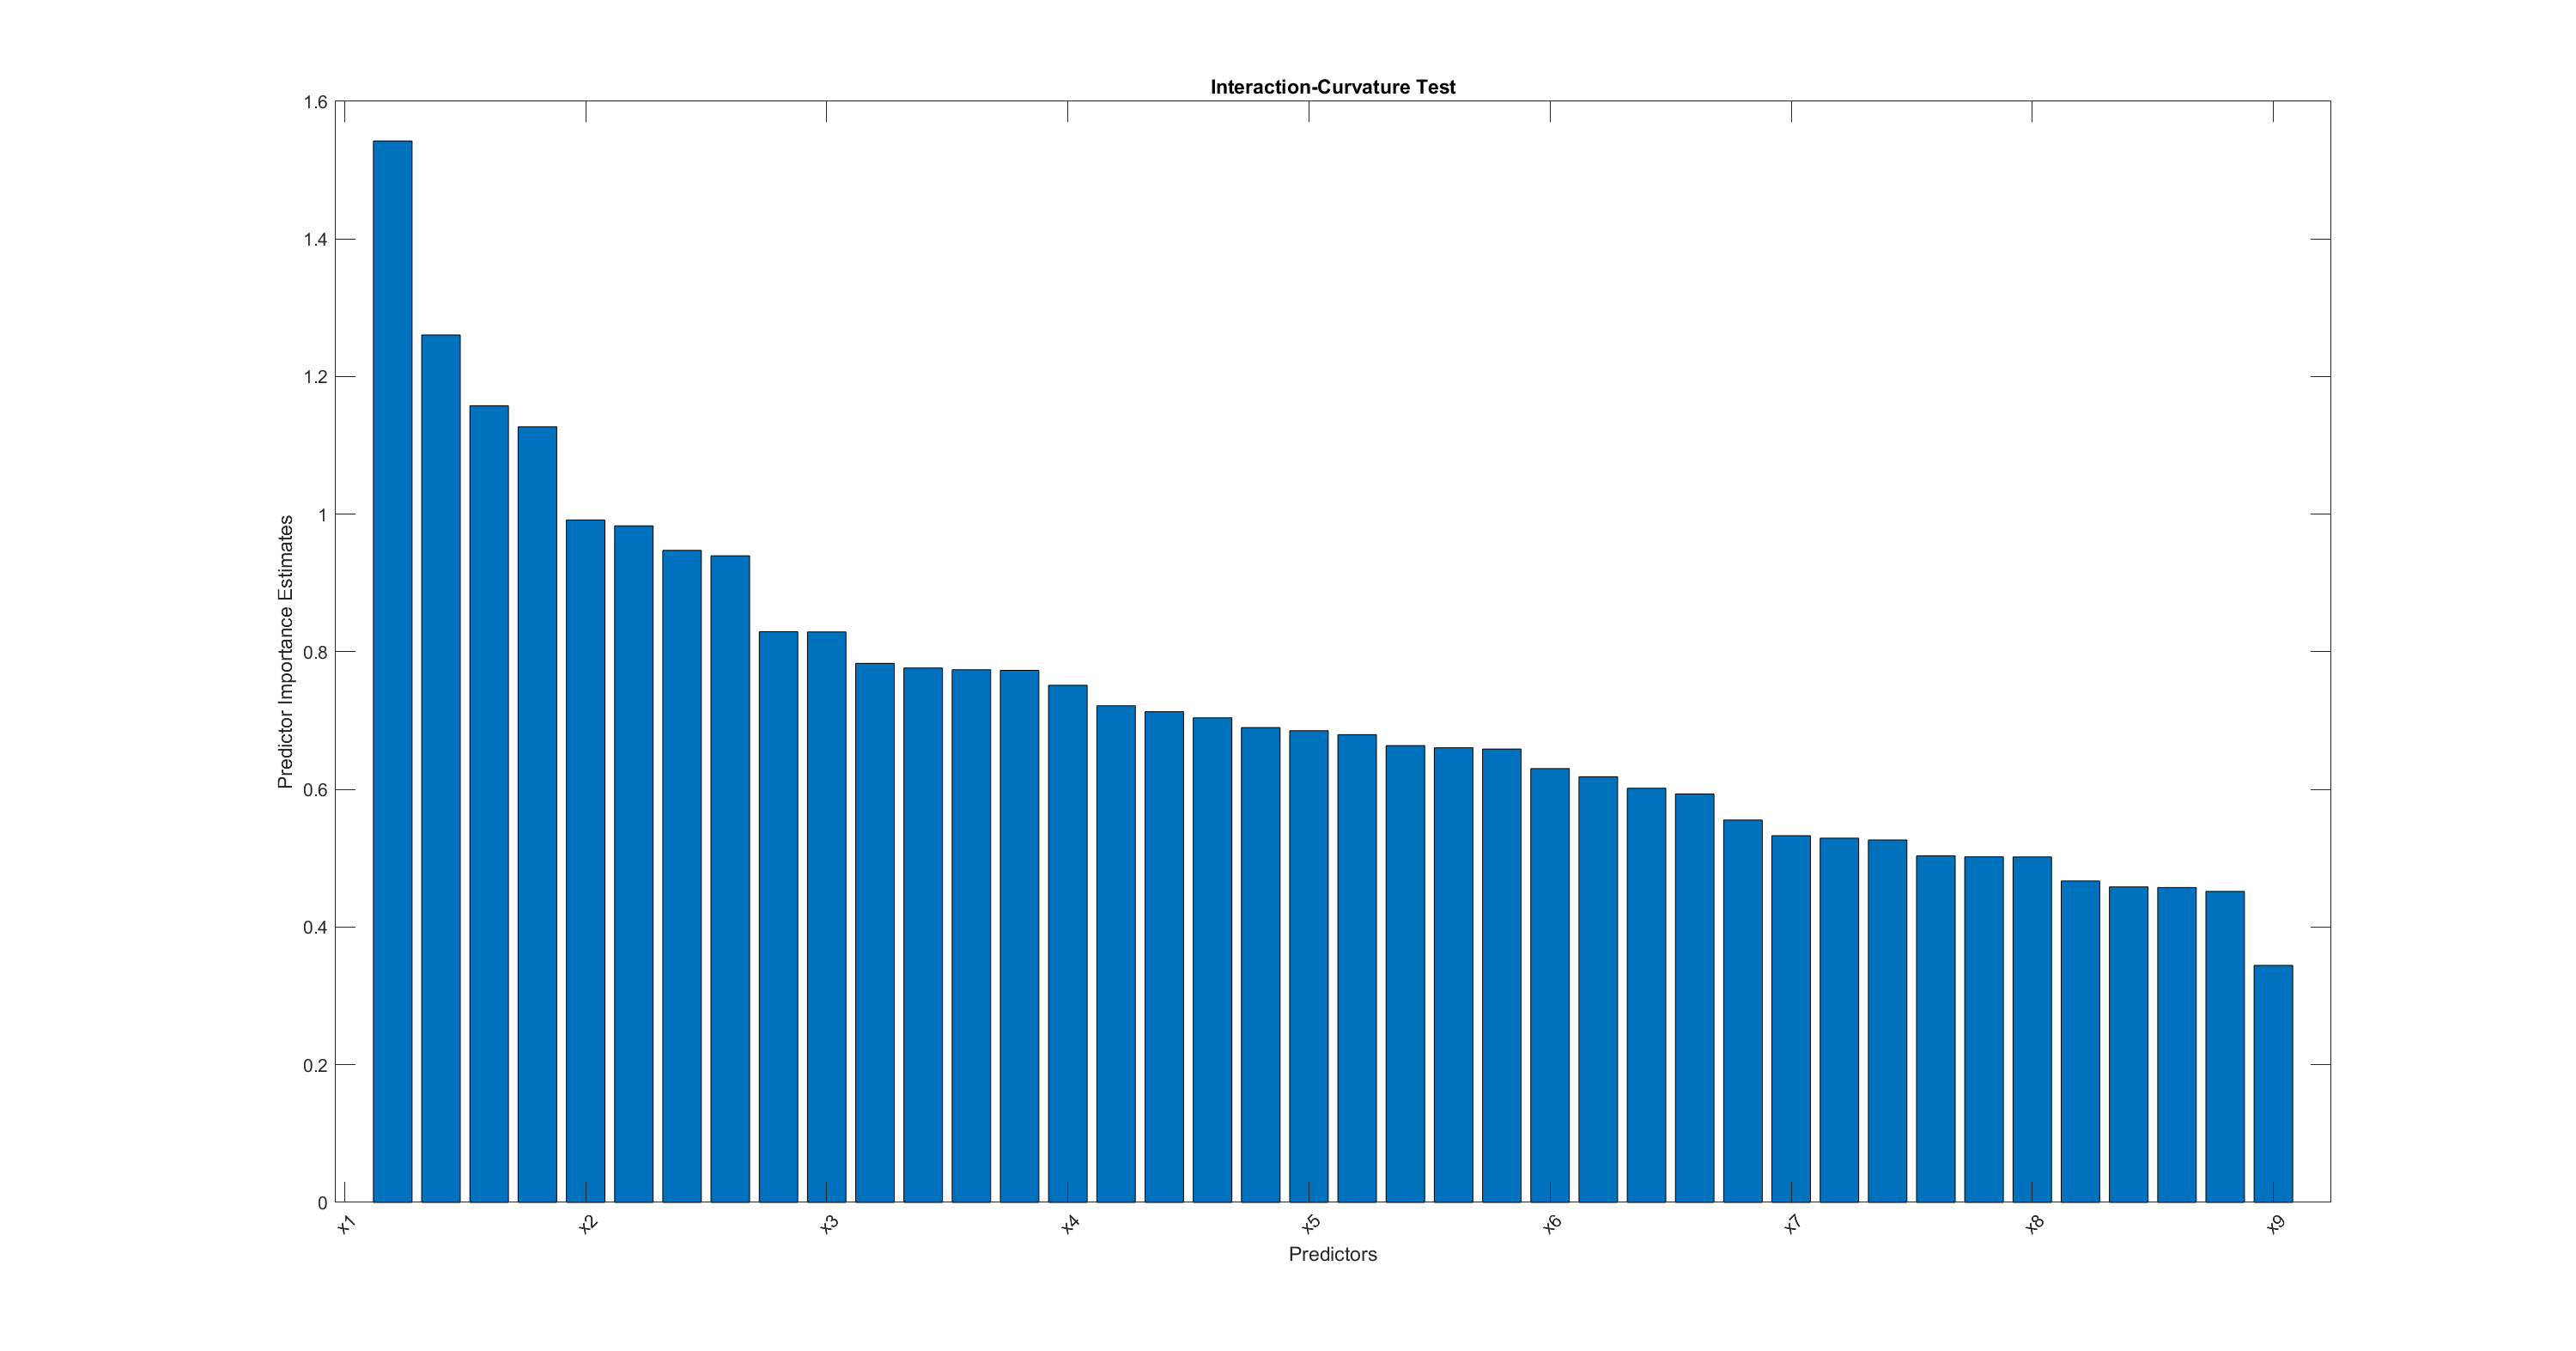
\includegraphics[width=1\textwidth]{images/importance_rf.png}
\caption{Predictors importance estimated by random forest after PCA}
\label{fig:myimage}
\end{figure}

By analysing the figure above, we can come to the conclusion that the number 8 is indeed a reasonable number for the final dimension of the feature space, after feature selection/reduction. Below those top 8 features, the remaining have a relatively low importance, according to the Random Forest algorithm.

\section{Classifiers}
In this section we will discuss the Minimum Distance Classifier with several distance formulas, to find out which one is more suitable for this problem.

\subsection{Minimum Distance Classifier}

A minimum distance classifier is a type of classification algorithm that assigns a test sample to the class with the closest mean or centroid. It works by computing the distance between the test sample and the means of each class, and then assigning the test sample to the class with the minimum distance.

The minimum distance classifier is often used in pattern recognition applications, and is relatively simple and computationally efficient. However, it assumes that the class distributions are Gaussian and have equal covariance matrices, which may not always hold true in practice. Additionally, it can suffer from class overlap, where samples from different classes may have similar mean vectors or centroids, leading to misclassifications.
In a minimum distance classifier, many distance metrics can be used to compute the distance between the test sample and the mean of each class. Some commonly used distance metrics include Euclidean distance, Mahalanobis distance, and cosine distance, among others. The used distance metrics are listed below.

\subsubsection{Euclidean Distance}


\begin{align}
d(\boldsymbol{x},\boldsymbol{y}) = ||\boldsymbol{x} - \boldsymbol{y}||2 = \sqrt{\sum{i=1}^n (x_i - y_i)^2}
\end{align}

where $n$ is the number of dimensions (features) in the feature space.

\subsubsection{Cityblock Distance}

\begin{align}
d(\boldsymbol{x},\boldsymbol{y}) = \sum_{i=1}^n |x_i - y_i|
\end{align}

where $n$ is the number of dimensions (features) in the feature space.

\subsubsection{Minkowski Distance}

\begin{align}
d(\boldsymbol{x},\boldsymbol{y}) = \left(\sum_{i=1}^n |x_i - y_i|^p\right)^{\frac{1}{p}}
\end{align}

where $p$ is a parameter that controls the degree of norm. When $p=1$, this distance metric is the cityblock distance. When $p=2$, it is the Euclidean distance.

\subsubsection{Chebychev Distance}

\begin{align}
d(\boldsymbol{x},\boldsymbol{y}) = \max_{i=1,\dots,n} |x_i - y_i|
\end{align}

This distance metric measures the maximum difference between any feature in the two feature vectors.

\subsubsection{Mahalanobis Distance}

\begin{align}
d(\boldsymbol{x},\boldsymbol{y}) = \sqrt{(\boldsymbol{x} - \boldsymbol{y})^T\boldsymbol{S}^{-1}(\boldsymbol{x} - \boldsymbol{y})}
\end{align}
where $\boldsymbol{S}$ is the covariance matrix of the feature space. This distance metric takes into account the correlation between the features in the feature space.

\vspace{1cm}

This distance is a useful metric in machine learning and pattern recognition techniques for several reasons:

It takes into account the correlation between features: Unlike Euclidean distance, which treats each feature as independent, Mahalanobis distance considers the covariance matrix of the features. This means that if two features are highly correlated, their contribution to the distance will be reduced, leading to more accurate clustering and classification.

It can handle data with different scales: In Mahalanobis distance, each feature is normalized by its variance. This means that features with larger variances will have a smaller contribution to the distance, which ensures that no feature dominates the distance calculation.

It can identify outliers: Mahalanobis distance can be used to detect outliers in the data because it considers the covariance structure of the data. Outliers tend to have a larger Mahalanobis distance from the center of the data distribution, which makes them easier to detect.

In the context of this project, Mahalanobis distance may be a promising option to use if the data have correlated features and/or features with different scales. It can help to improve the accuracy of clustering and classification models and identify outliers in the data. However, it's important to note that Mahalanobis distance can be computationally expensive for large datasets, so it may not be feasible for some projects.

\section{Results}

We tested three different normalization techniques and five different distance formulas for the classifiers, as mentioned before, to see which one would perform better in a Binary Classification scenario.

In the next figures we can see the validation results of this experiment, in which we computed five different performance measures:

\begin{itemize}
    \item Mean-Squared Error (MSE)
    MSE = $\frac{1}{n} \sum_{i=1}^{n}(y_i - \hat{y_i})^2$
    \item Accuracy
    Accuracy =  $\frac{TP + TN}{TP + TN + FP + FN}$
    \item Specificity 
    Specificity = $\frac{TN}{TN + FP}$
    \item Sensitivity
    Sensitivity= $\frac{TP}{TP + FN}$
    \item F-measure
    $F_{\beta} = (1 + \beta^2) \frac{precision \times recall}{(\beta^2 \times precision) + recall}$

    \vspace{0.5cm}
    \small{Note that recall = sensitivity.}
    
\end{itemize}

The results which we considered more interesting and showed a reasonable compromise between the five mentioned performance metrics are highlighted. It is important to note that in this context, the f-measure may be the most relevant performance metric since it takes into account the class imbalancing. This is due to the fact that it is computed as the harmonic mean of precision and recall, with a higher score indicating better performance in both precision and recall.

In the context of imbalanced datasets, as one ones used to feed the binary classificators, where one class has significantly fewer samples than the other(s), the F-measure can be a useful metric because it gives equal weight to precision and recall. 

However, in some csas, the F-measure does not always compensate for class imbalabcing. There are several alternatives to it that take into account class imbalancing. One such measure is the balanced accuracy, which is the arithmetic mean of the sensitivity and specificity of a classifier. Another measure is the geometric mean, which is the square root of the product of the sensitivity and specificity. Both of these measures give equal weight to each class, regardless of the class distribution.

Another commonly used measure for imbalanced datasets is the area under the receiver operating characteristic curve (AUC-ROC), which measures the trade-off between true positive rate and false positive rate. This measure is often used when the goal is to maximize the true positive rate while keeping the false positive rate low.

The above-mentioned performance metrics may be explored in future work of this project.

\vspace{1cm}

\begin{figure}[H]
\centering
\includegraphics[width=1\textwidth]{images/table1.png}
\caption{MDC performance metrics w/unit vector normalization}
\label{fig:myimage}
\end{figure}

\begin{figure}[H]
\centering
\includegraphics[width=1\textwidth]{images/table2.png}
\caption{MDC performance metrics w/min-max normalization}
\label{fig:myimage}
\end{figure}

\begin{figure}[H]
\centering
\includegraphics[width=1\textwidth]{images/table3.png}
\caption{MDC performance metrics w/zscore normalization}
\label{fig:myimage}
\end{figure}

\small{
\begin{itemize}
    \item 
     MSE - Mean Squared Error
    \item 
     acc - accuracy
    \item 
     spec - specificity
    \item 
     sens - sensitivity
    \item 
     f - f-measure
\end{itemize}
}

 We can deduce that the "Classical" genre is the easiest class to classify, as it has the best results overall, and the Mahalanobis distance is the metric for the Minimum Distance Classifier that overall presents better performance.

\vspace{1cm}
 Here we presented the performance of the MDC classifier on the training and validation sets, but did not provide results on the testing set. We made this decision because we want to properly build and store the classifiers for later testing with a separate dataset, which would allow for a more rigorous evaluation of the performance.

We acknowledged that the performance on the training and validation sets can provide valuable insights into the generalization capability of the highlighted classifiers. By evaluating the performance on the training and validation sets, we can determine how well the classifiers are able to learn and generalize to new examples from the same dataset.

However, we also noted that the performance on the training and validation sets may not necessarily reflect the performance on a separate testing set or real-world data. Therefore, it is important for us to test the classifiers on an independent dataset to evaluate their true performance.

Overall, the presented results provide a valuable first step in evaluating the performance of the classifiers on the GTZAN dataset, and further testing and evaluation will be necessary to fully assess their performance.

In the next figures, we can see the confusion matrices for the eight most promising combinations of Class + Normalization + Distance Metric, which correspond to a binary minimum-distance classifier. As said before, these confusion matrices are related to the training/validation phase.

\begin{figure}[H]
\centering
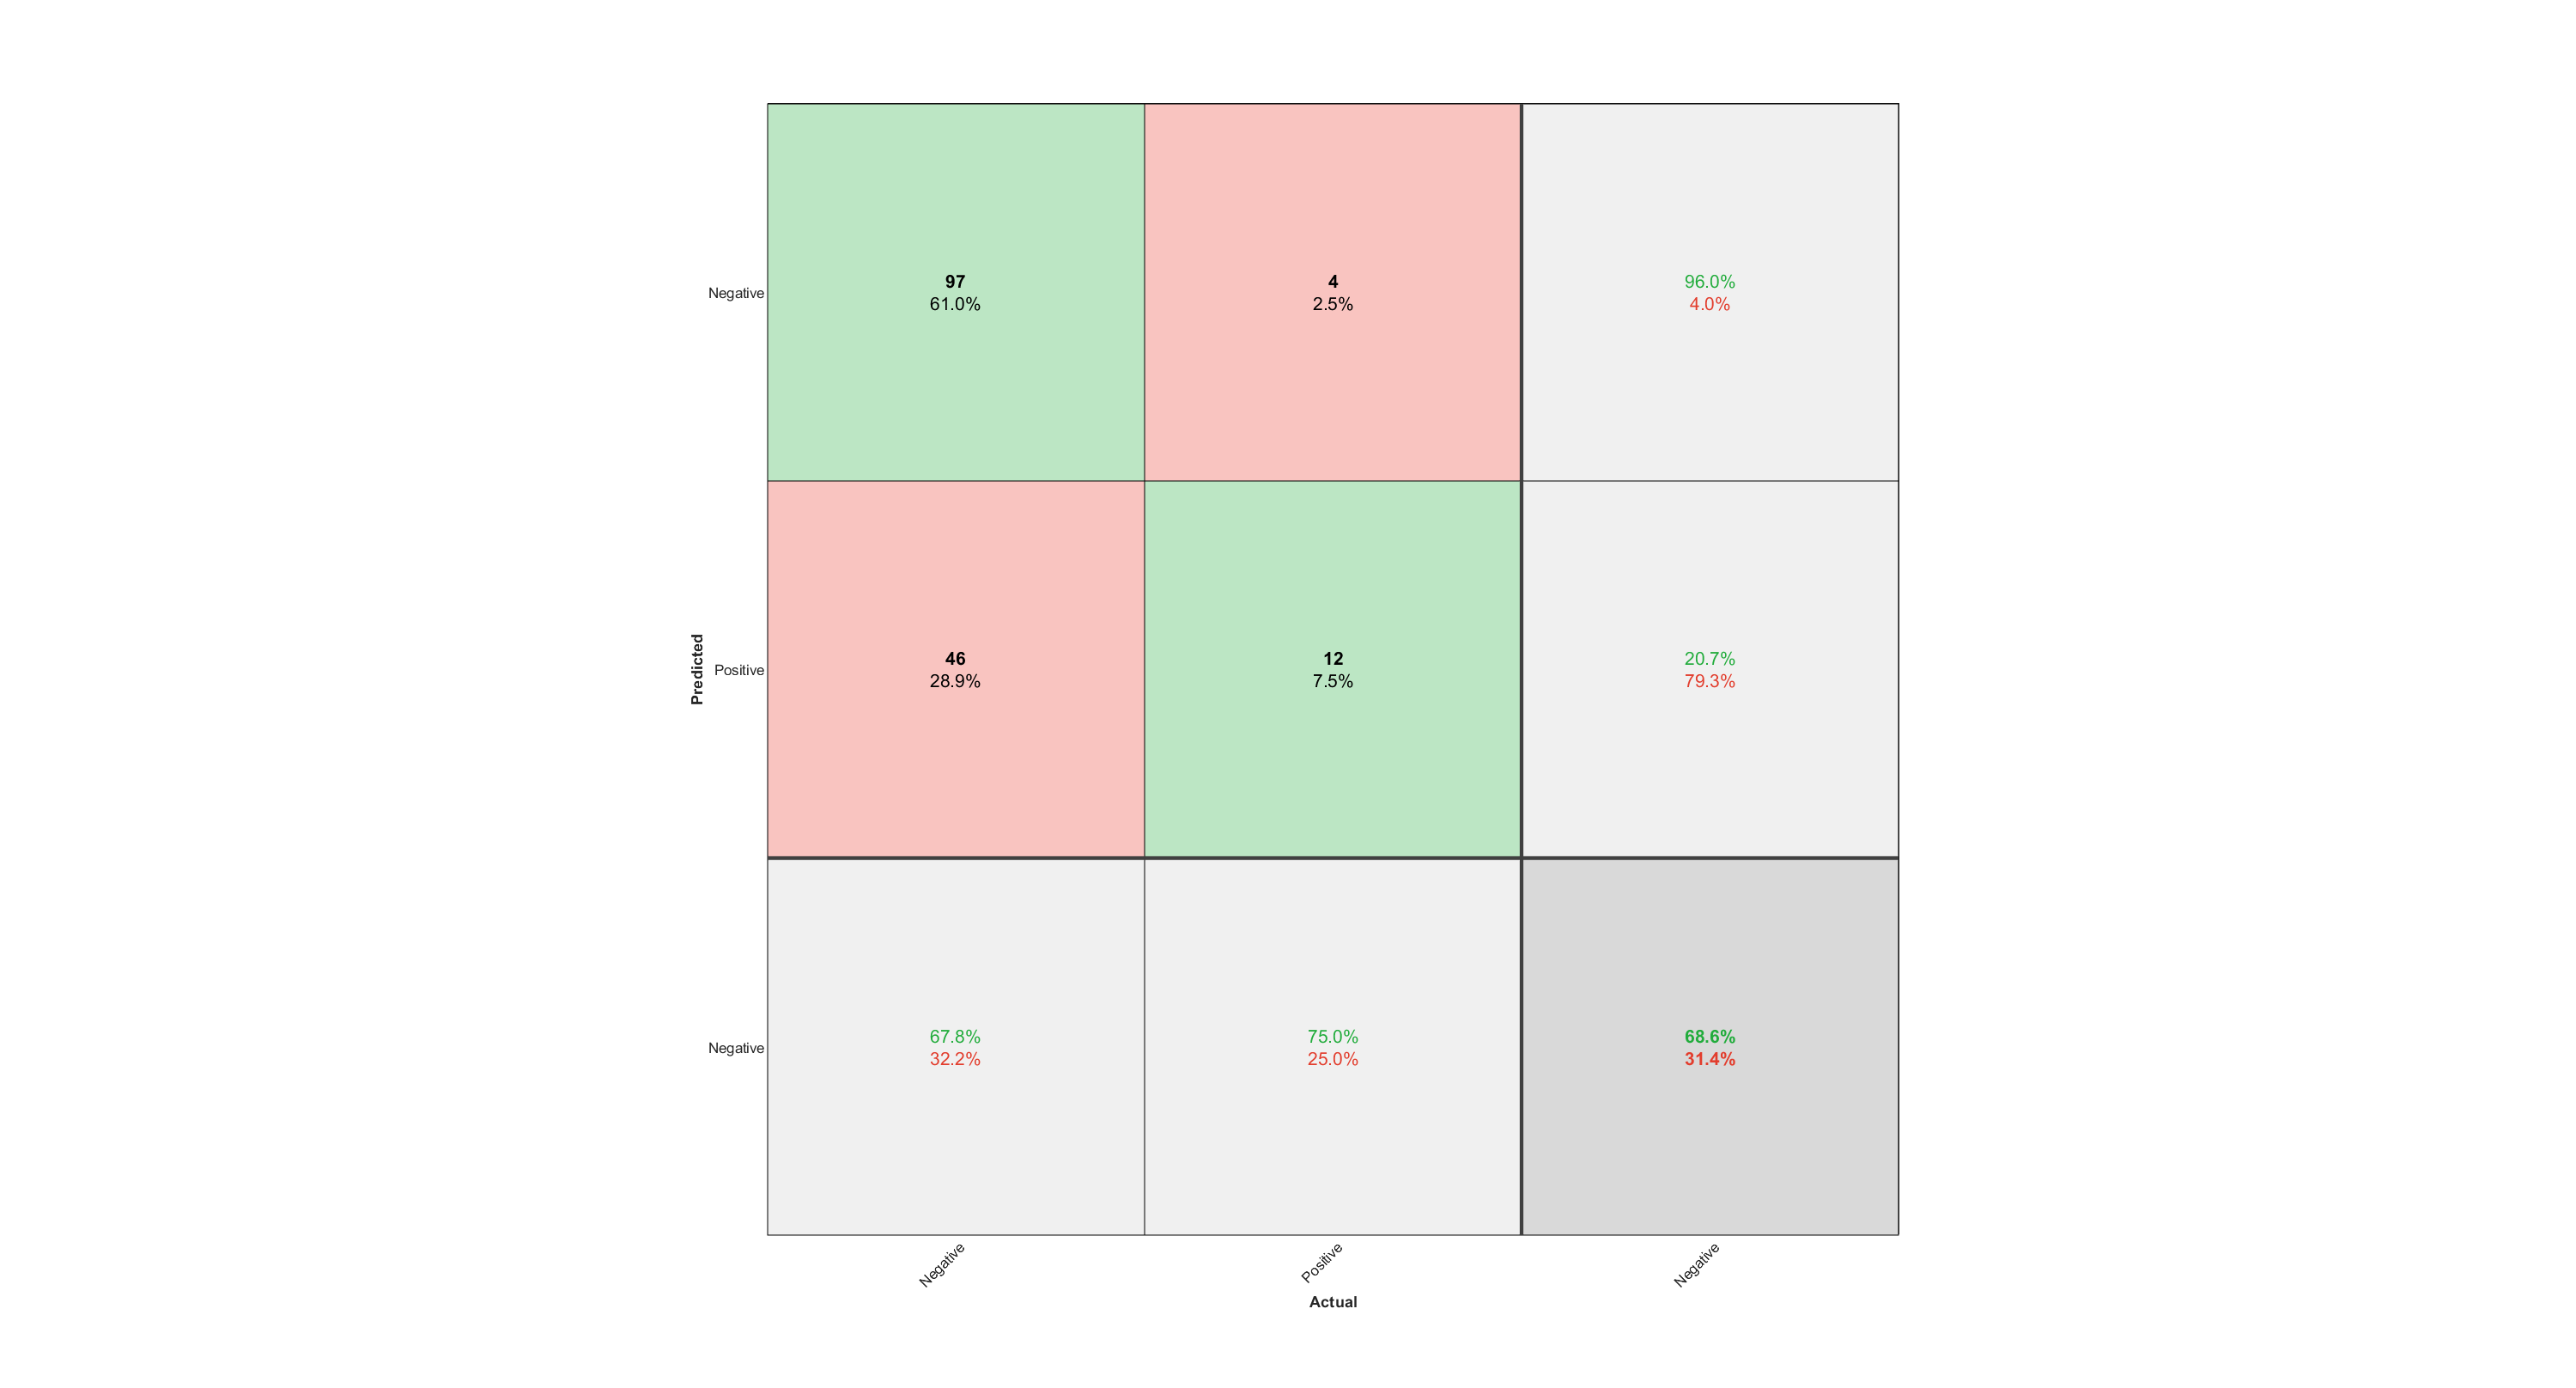
\includegraphics[width=1\textwidth]{images/cm_blues_norm_mahalanobis.png}
\caption{Blues + Unit Vector + Mahalanobis}
\label{fig:myimage}
\end{figure}

\begin{figure}[H]
\centering
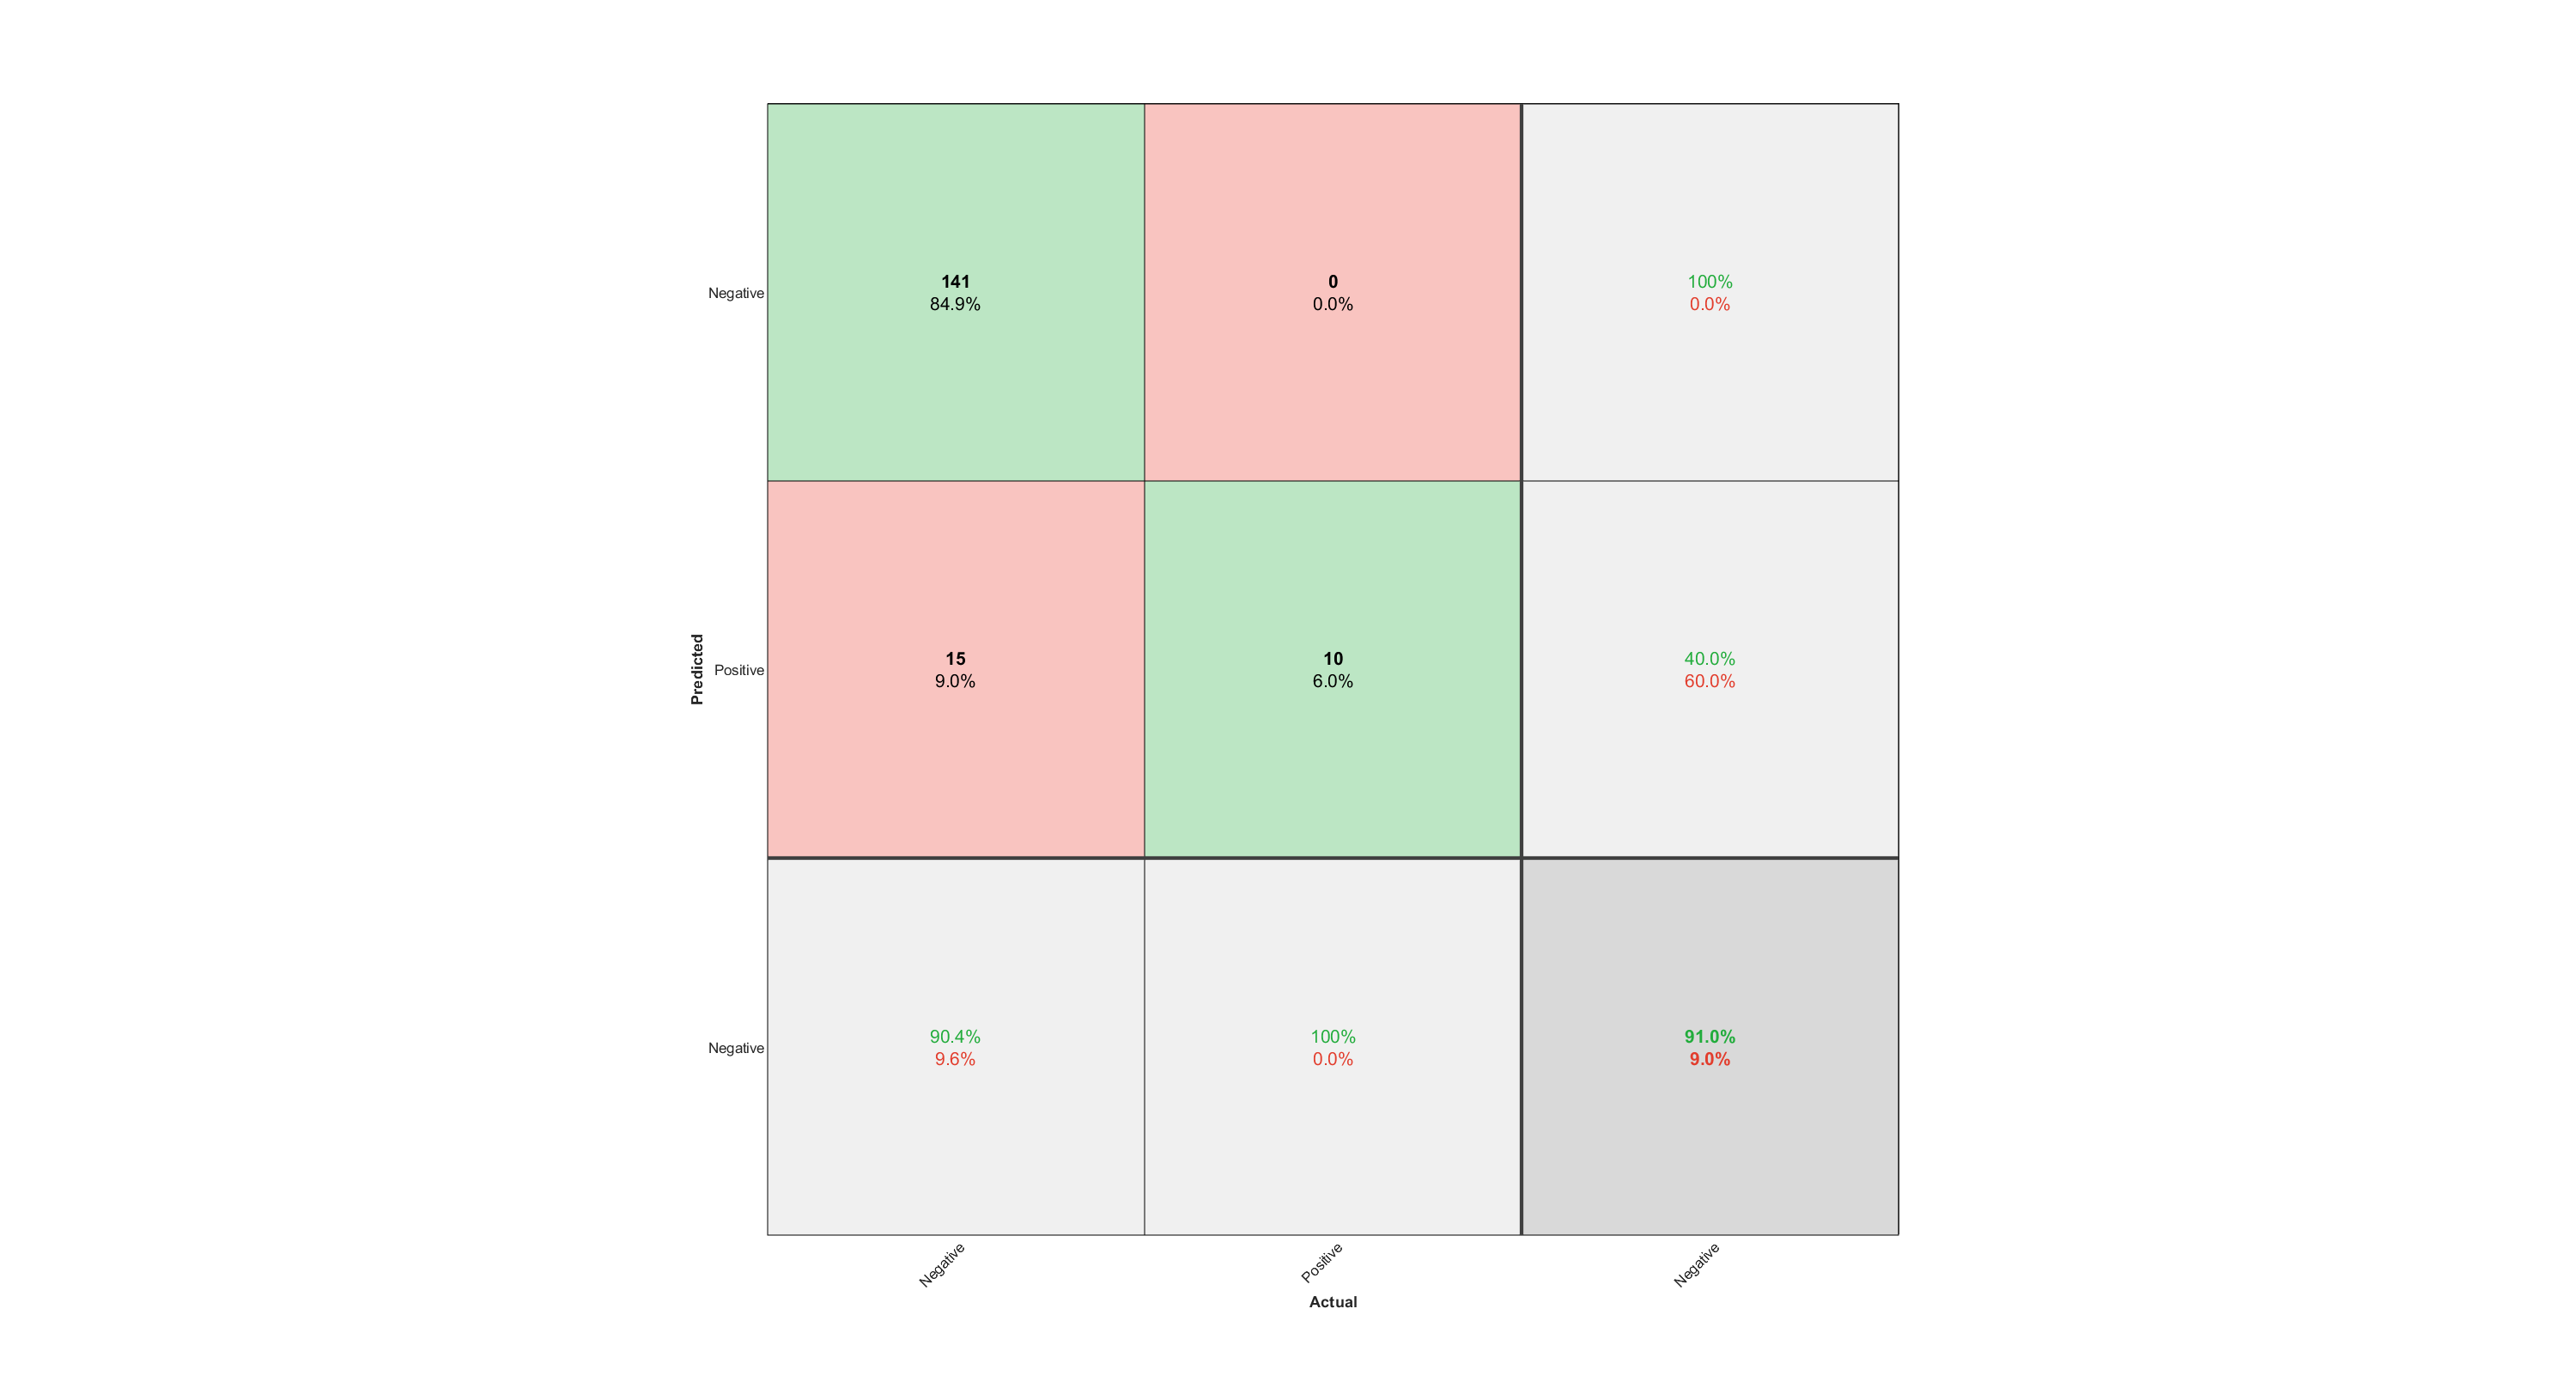
\includegraphics[width=1\textwidth]{images/cm_classical_range_cityblock.png}
\caption{Classical + Range + CityBlock}
\label{fig:myimage}
\end{figure}

\begin{figure}[H]
\centering
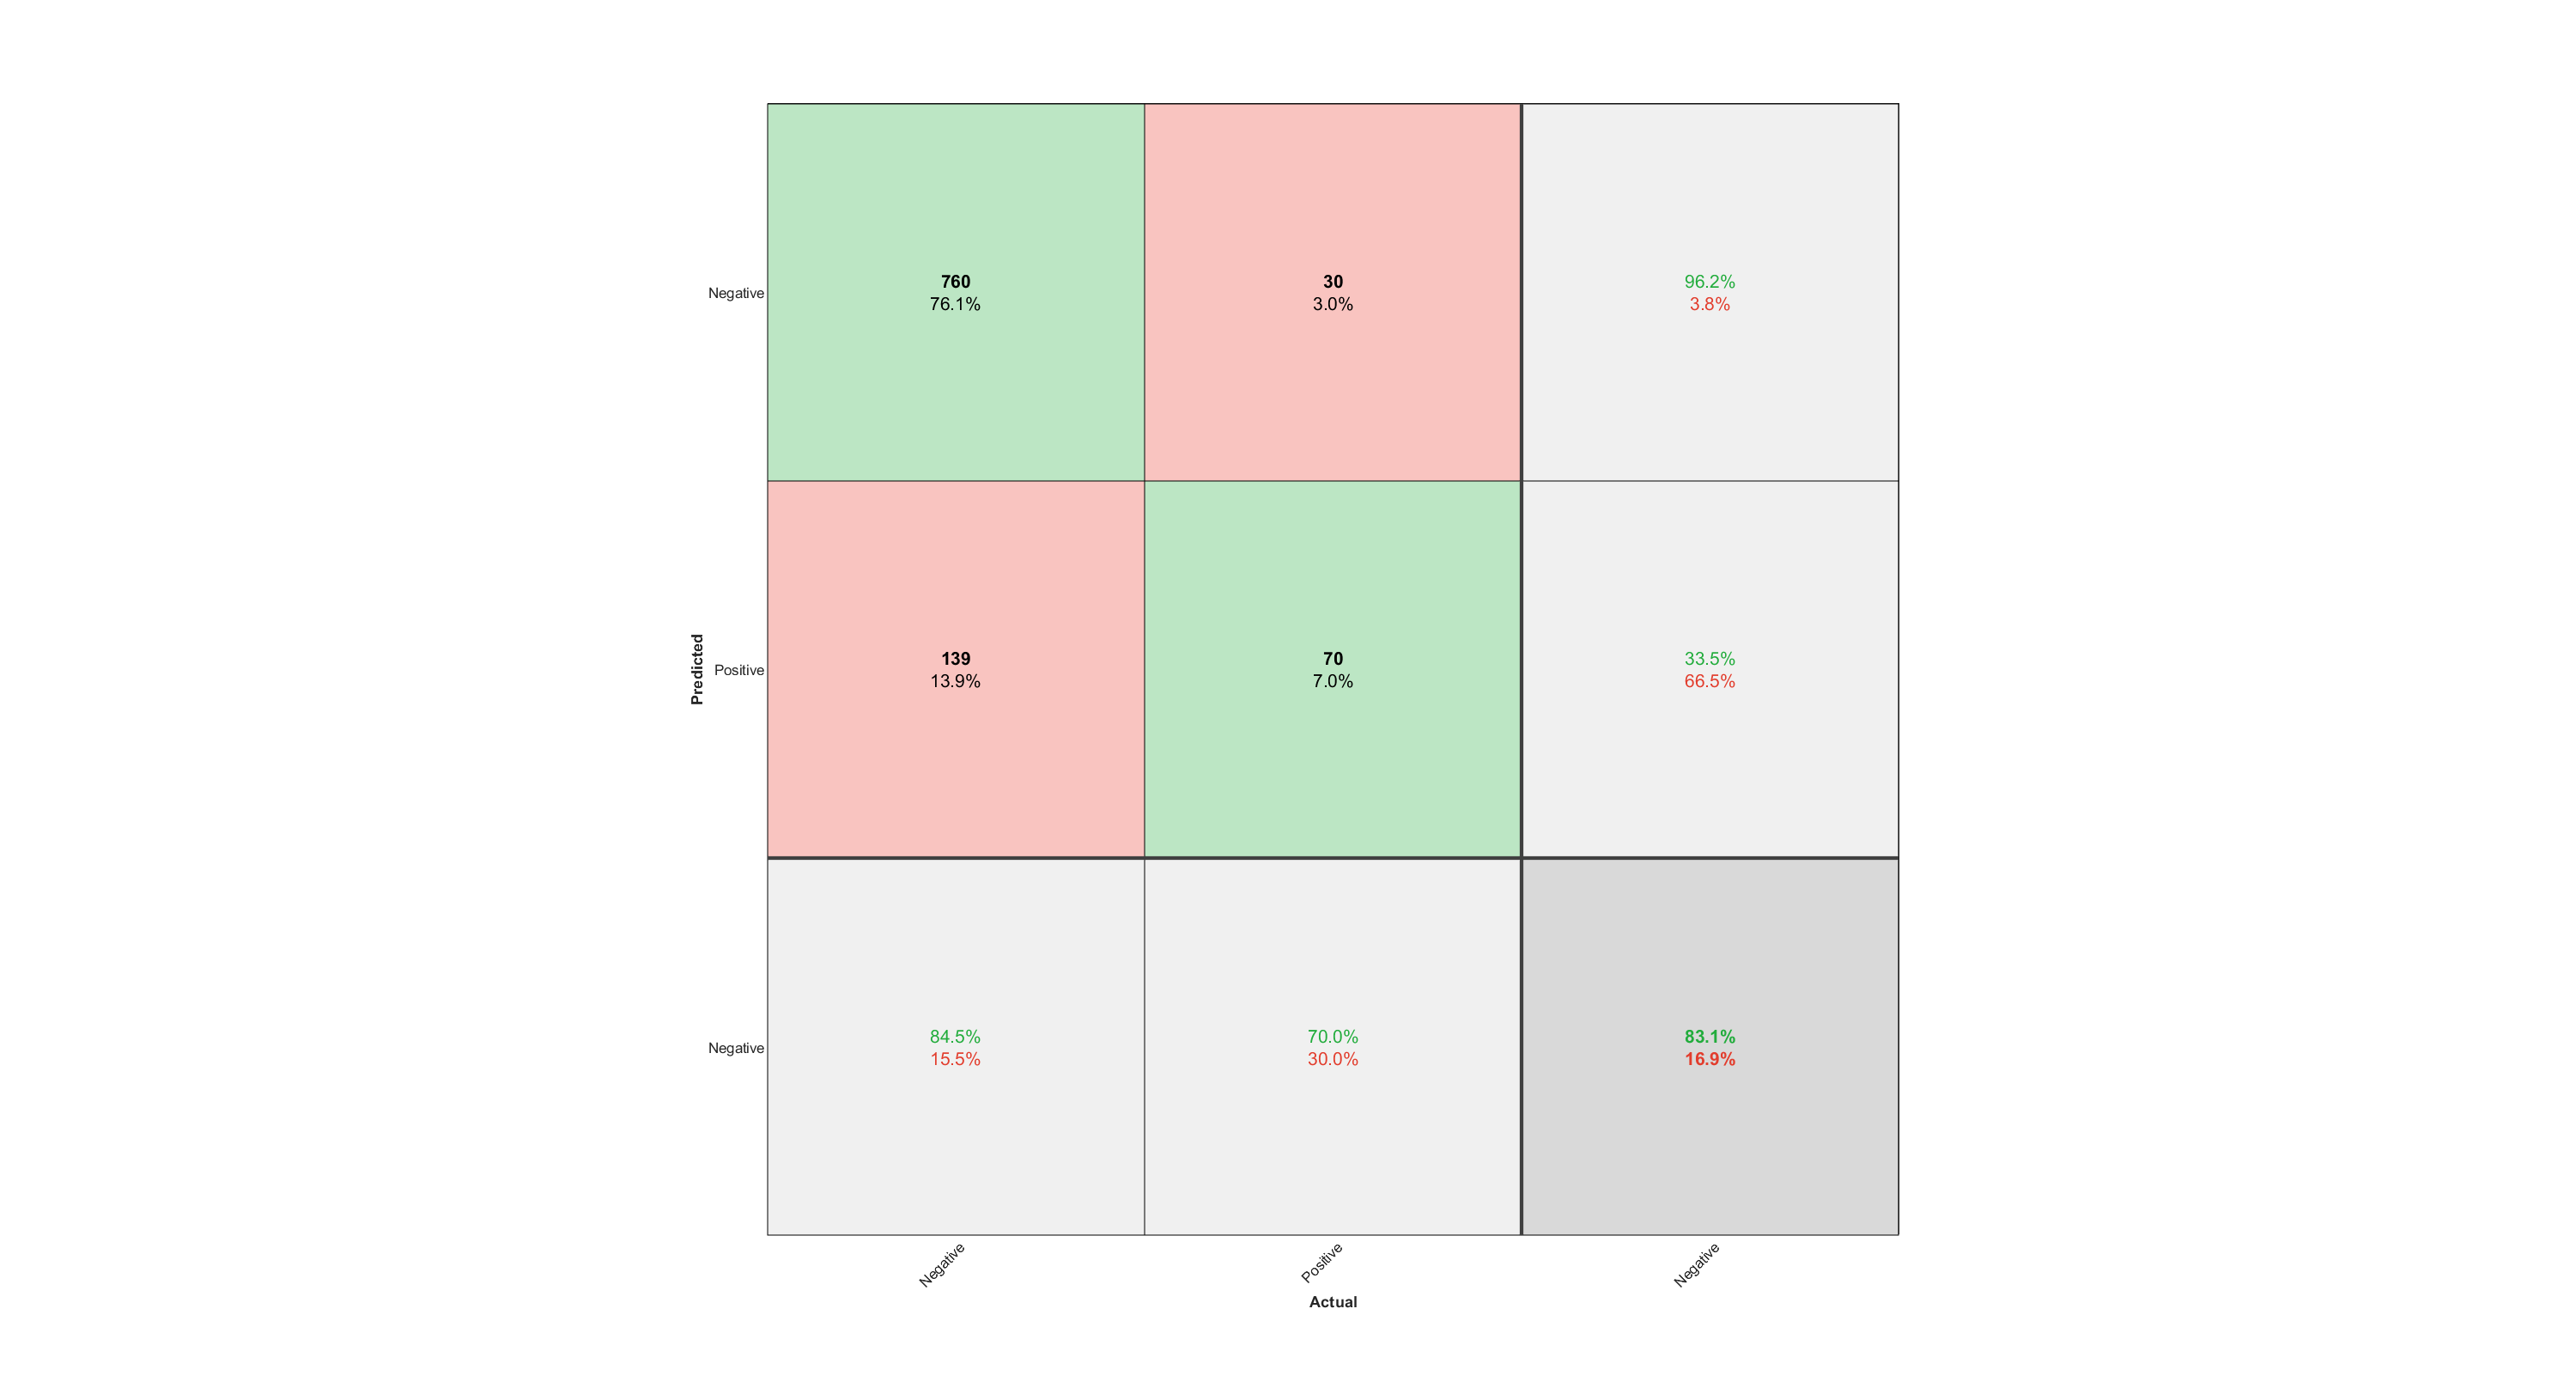
\includegraphics[width=1\textwidth]{images/cm_classical_range_euclidean.png}
\caption{Classical + Range + Euclidean}
\label{fig:myimage}
\end{figure}

\begin{figure}[H]
\centering
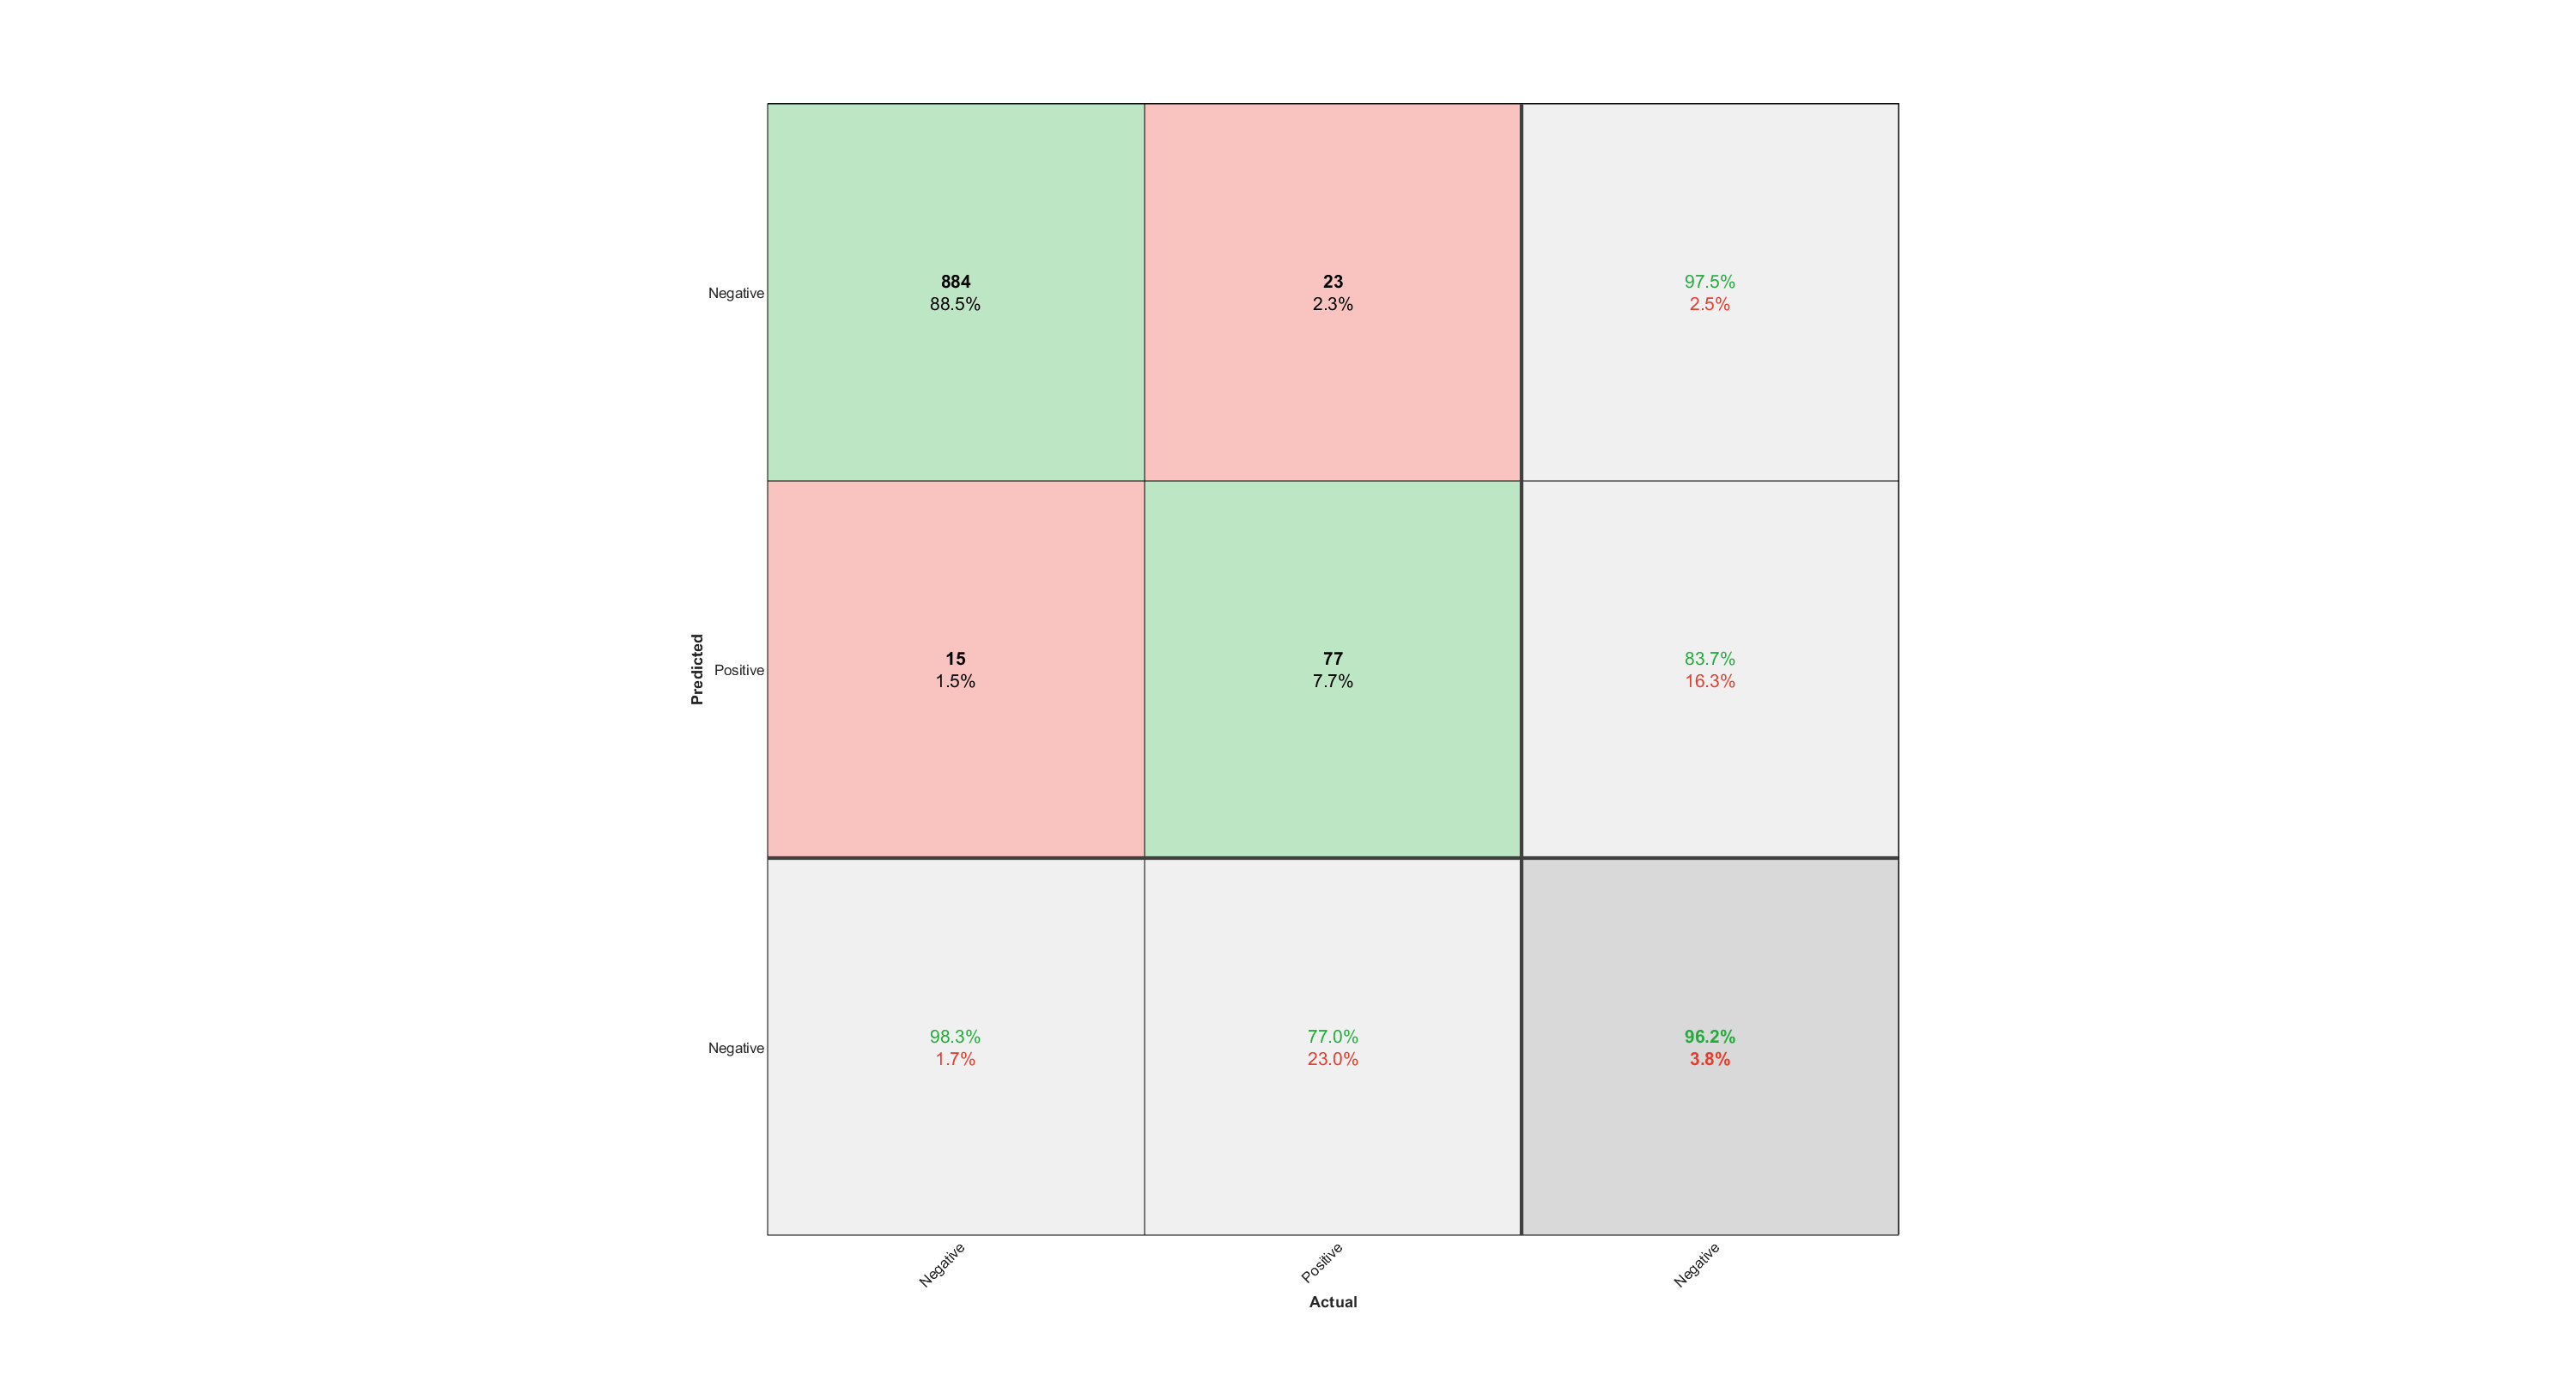
\includegraphics[width=1\textwidth]{images/cm_classical_range_mahalanobis.png}
\caption{Classical + Range + Mahalanobis}
\label{fig:myimage}
\end{figure}

\begin{figure}[H]
\centering
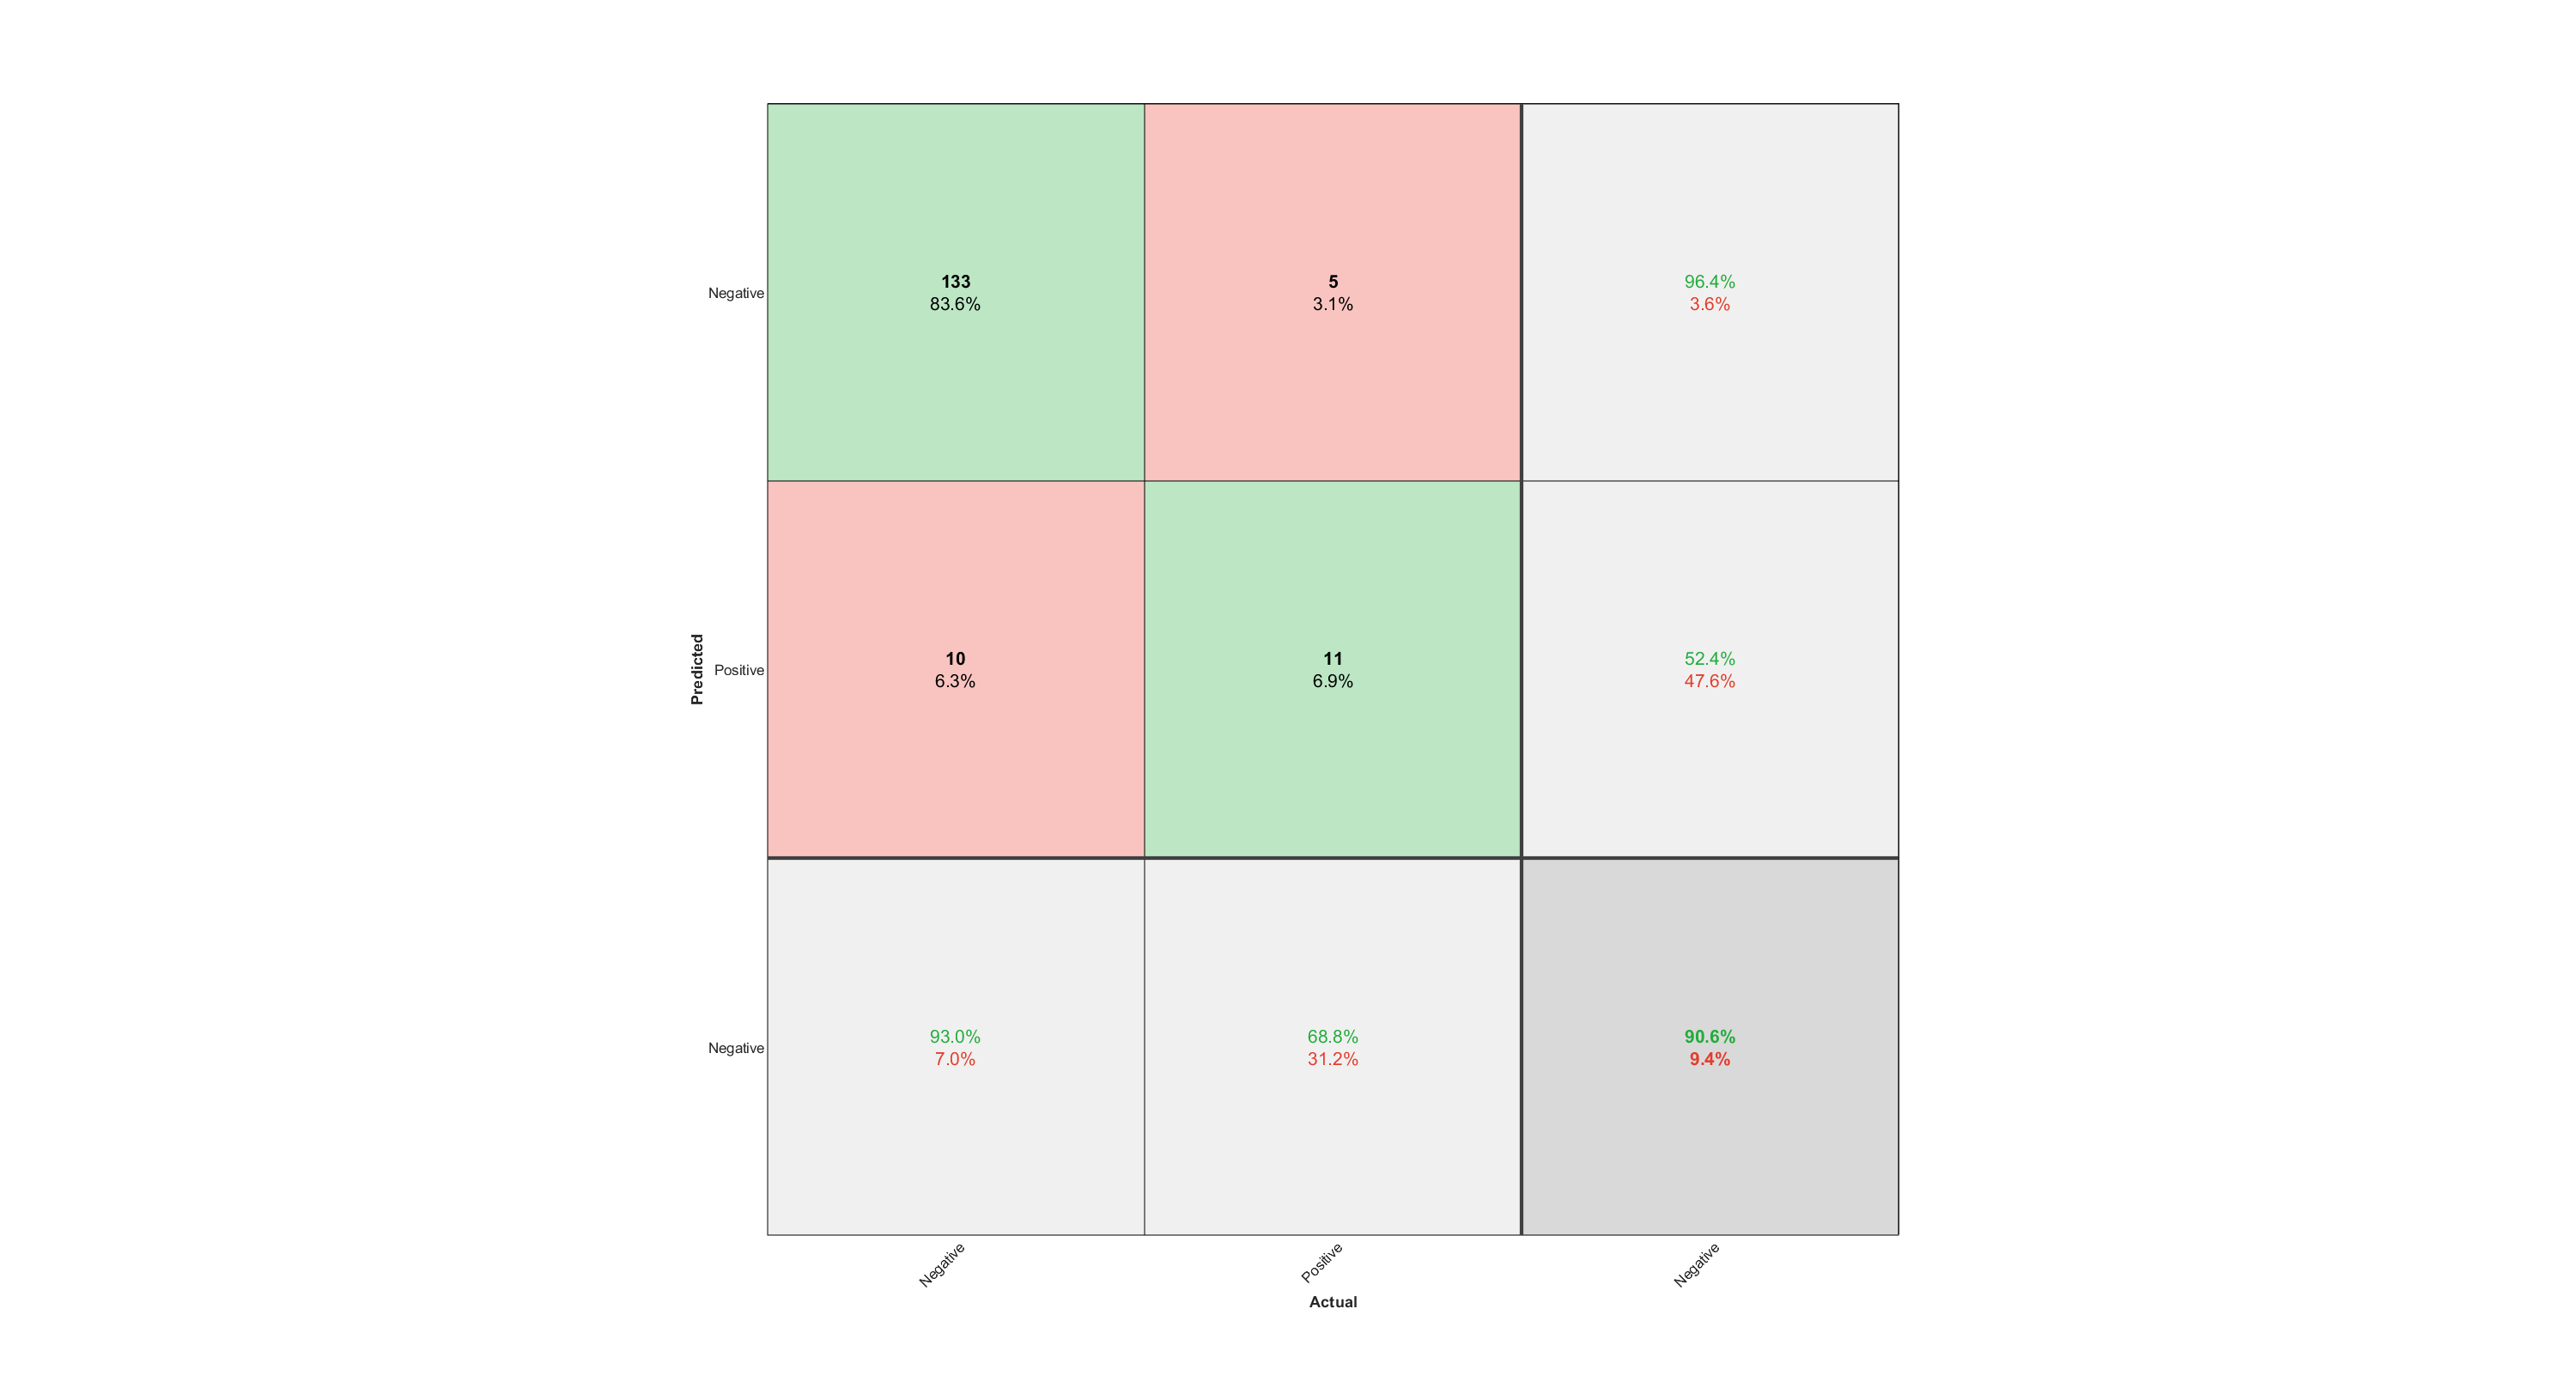
\includegraphics[width=1\textwidth]{images/cm_classical_zscore_minkowski.png}
\caption{Classical + zscore + Minkowski}
\label{fig:myimage}
\end{figure}

\begin{figure}[H]
\centering
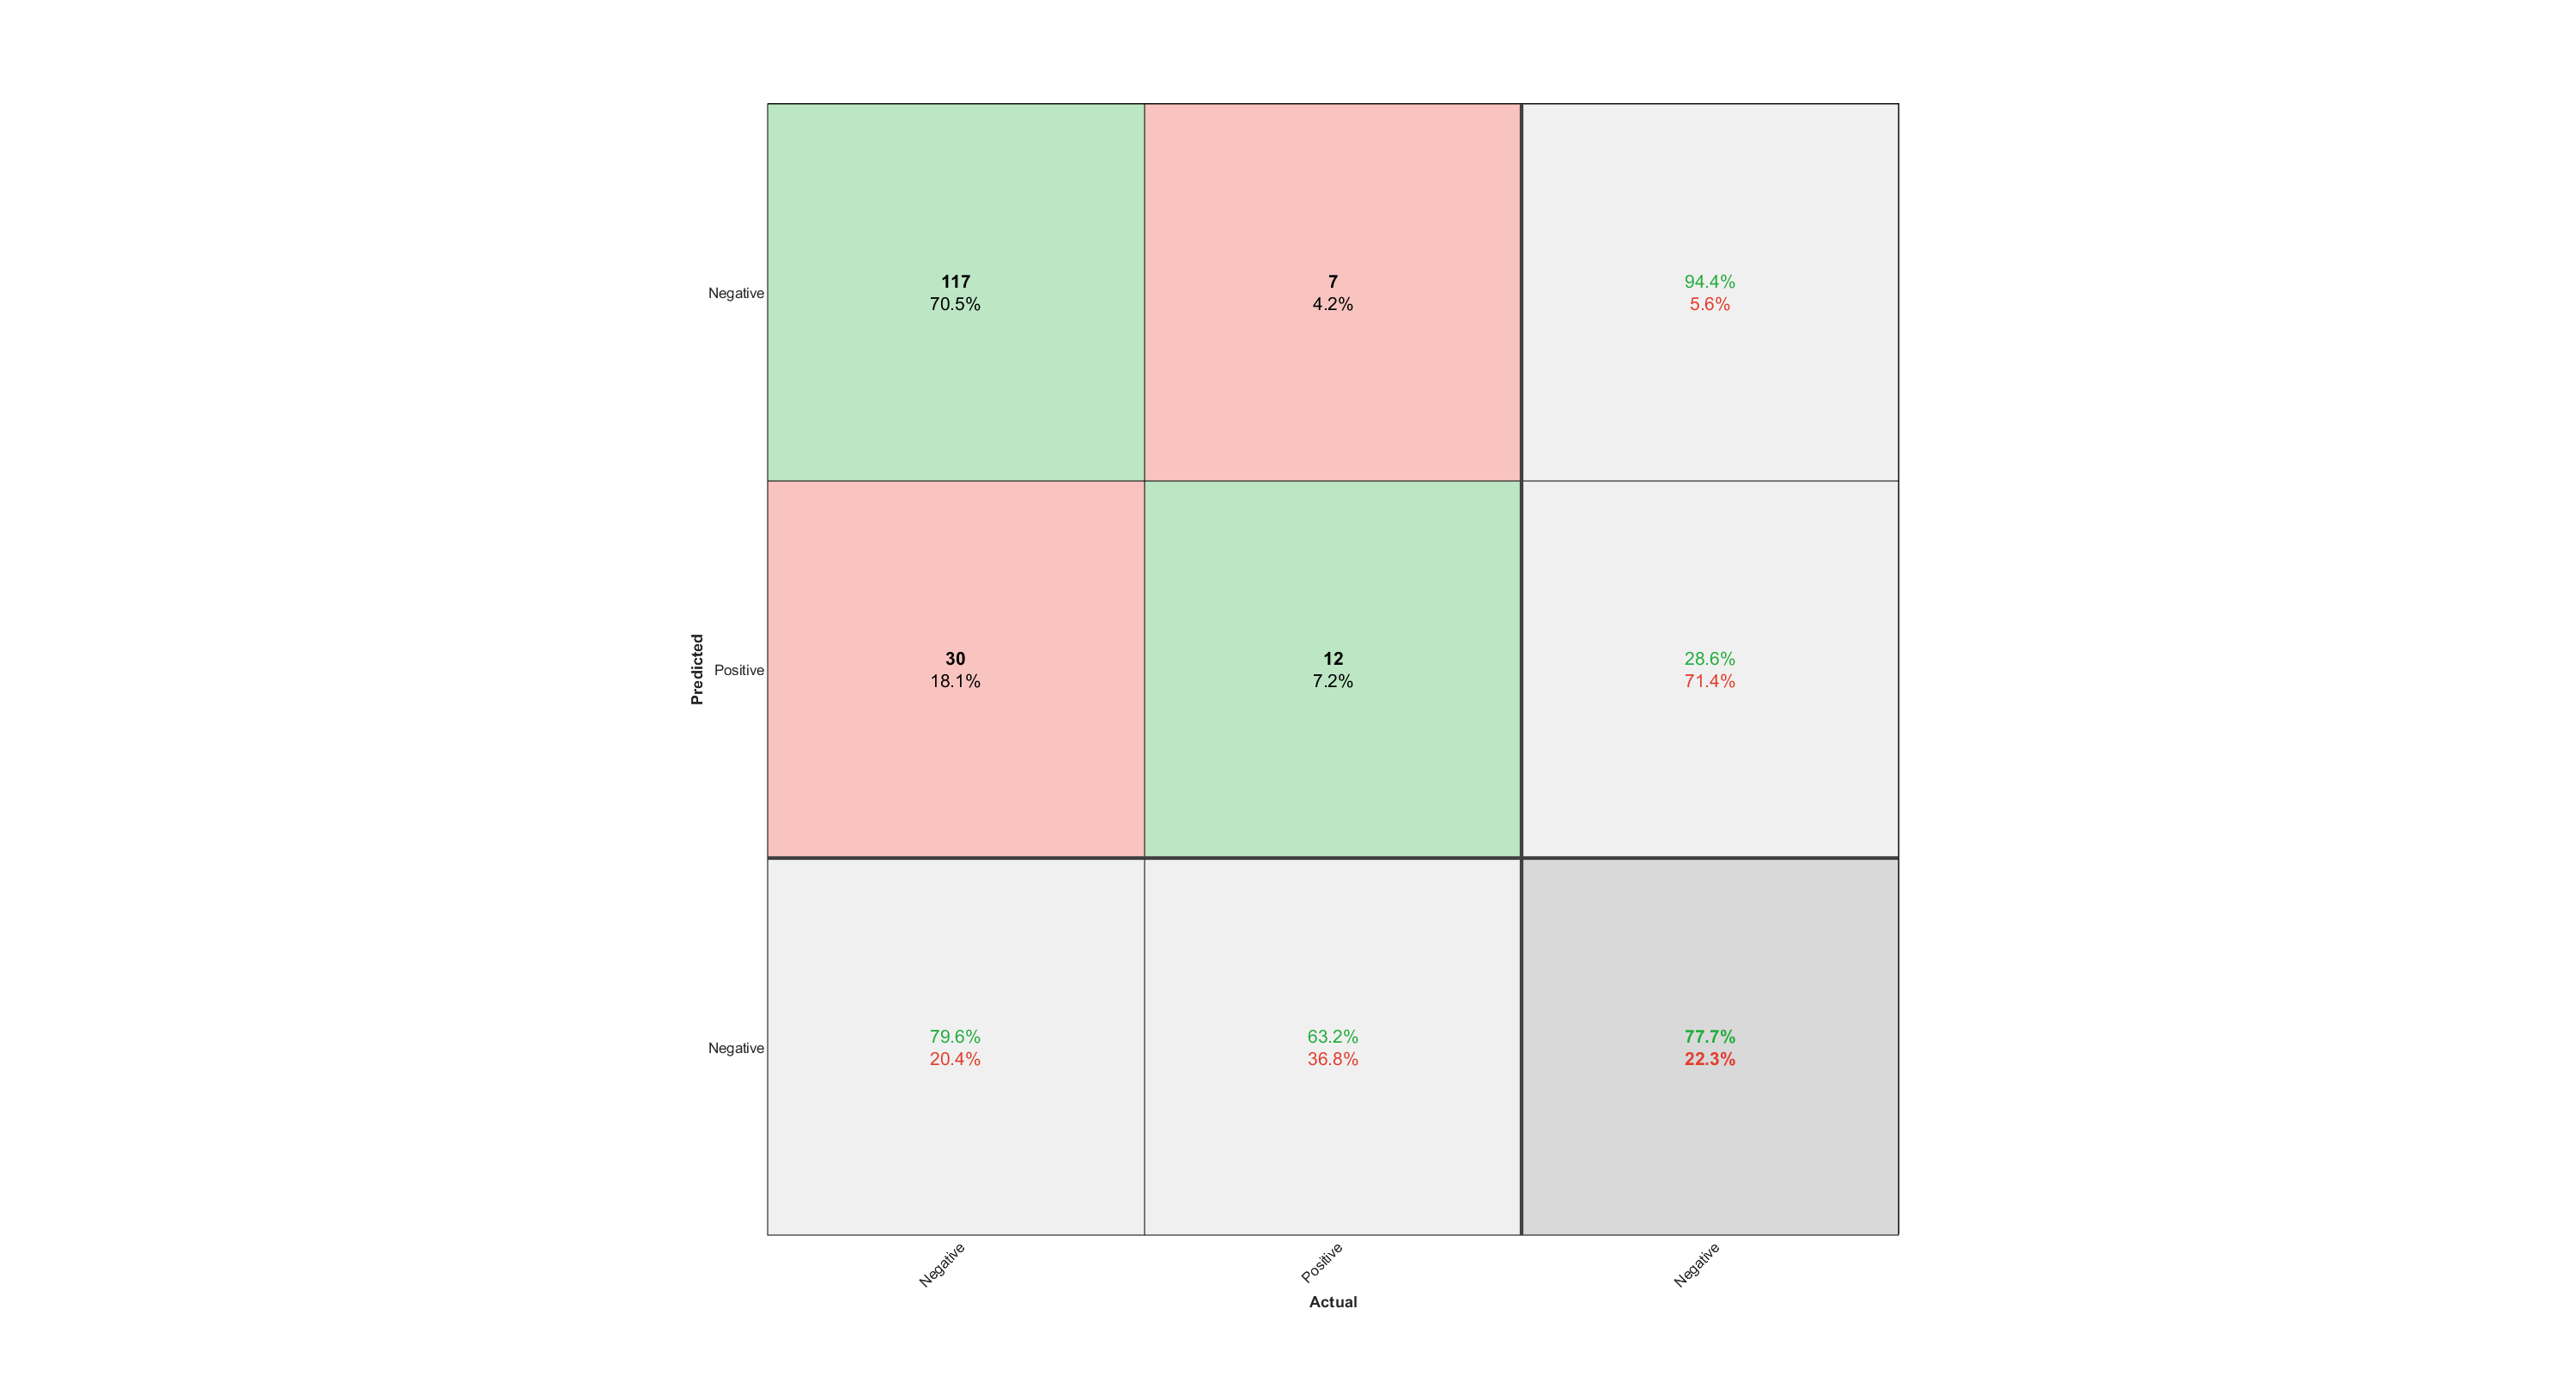
\includegraphics[width=1\textwidth]{images/cm_jazz_zscore_mahalanobis.png}
\caption{Jazz + zscore + Mahalanobis}
\label{fig:myimage}
\end{figure}

\begin{figure}[H]
\centering
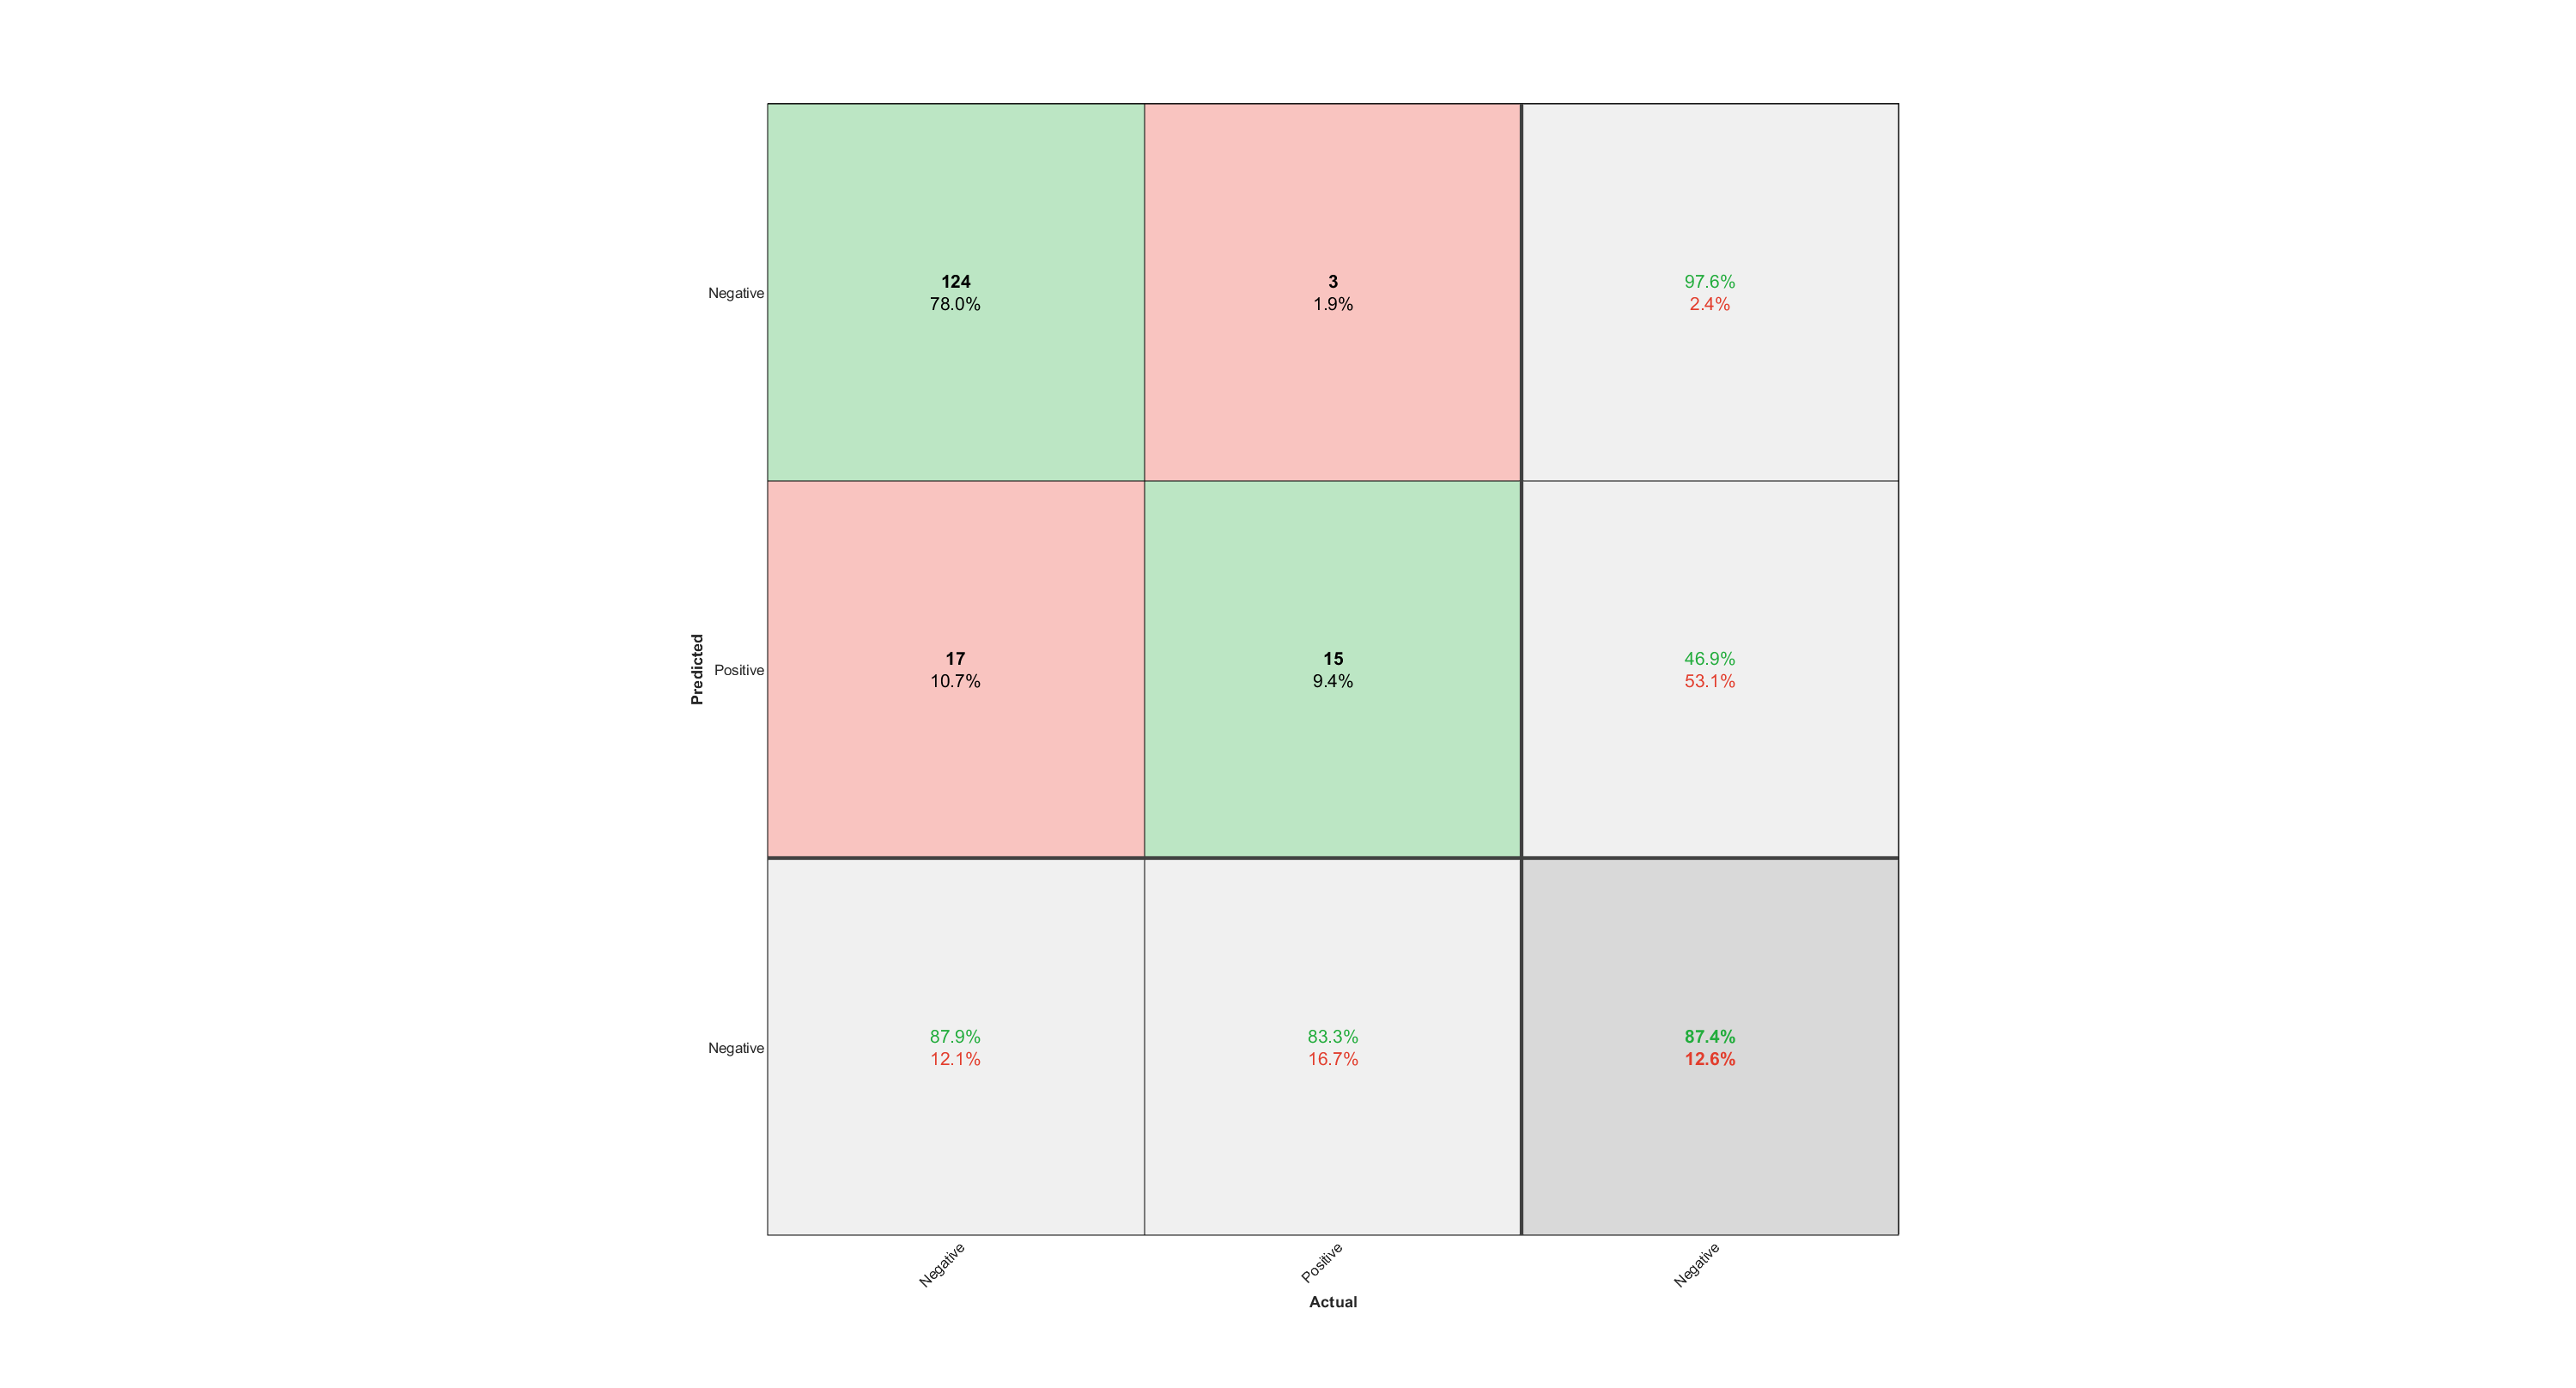
\includegraphics[width=1\textwidth]{images/cm_metal_norm_mahalanobis.png}
\caption{Metal + Unit Vector + Mahalanobis}
\label{fig:myimage}
\end{figure}

\begin{figure}[H]
\centering
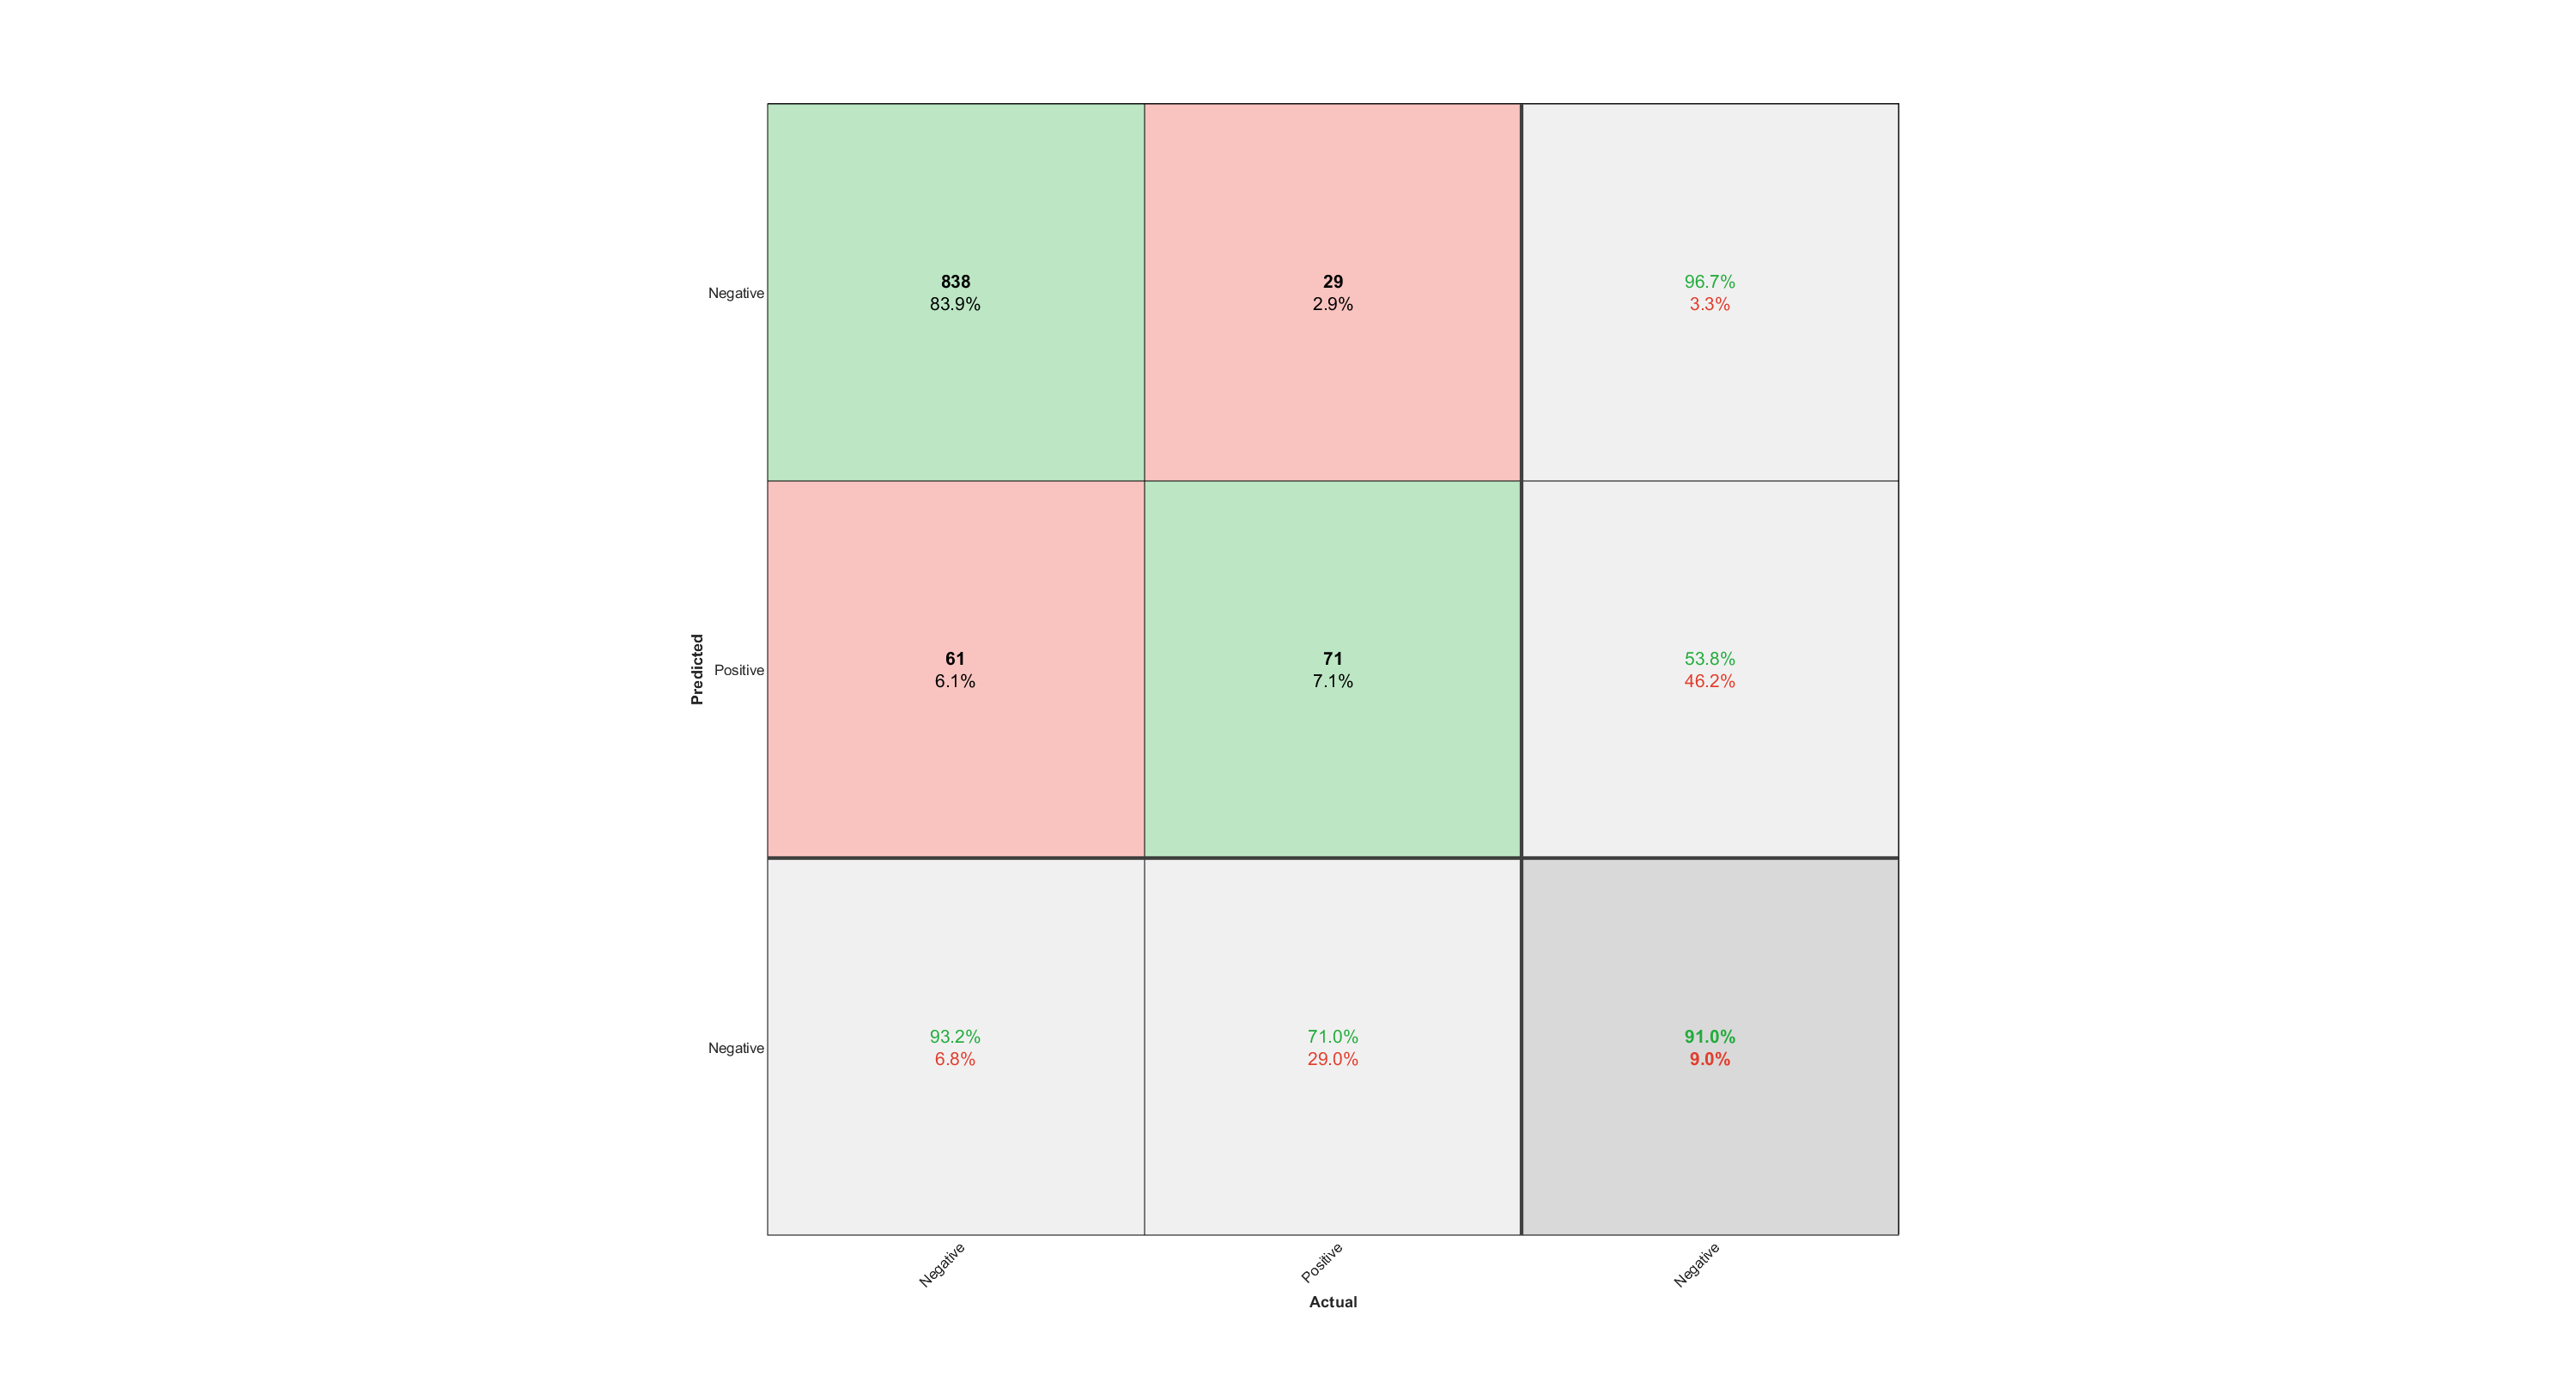
\includegraphics[width=1\textwidth]{images/cm_metal_zscore_mahalanobis.png}
\caption{Metal + zscore + Mahalanobis}
\label{fig:myimage}
\end{figure}

After analyzing the confusion matrices, it is evident that there is a significant class imbalance in the binary classification dataset. This imbalance is particularly noticeable when examining the percentages related to the true class (1) in the confusion matrix.

In binary classification, the confusion matrix is a table that summarizes the performance of a classification algorithm. It contains four possible outcomes: true positives (TP), false positives (FP), true negatives (TN), and false negatives (FN). The true positives and true negatives represent the correct classifications, while the false positives and false negatives represent the incorrect classifications.

When there is a class imbalance, it means that the number of samples in one class is significantly larger or smaller than in the other class. This can lead to poor performance of the classification algorithm because it may become biased towards the majority class.

In the context of the confusion matrix, the class imbalance is visible in the percentages related to the true class (1). For instance, if the dataset contains 90\% negative class (0) samples and only 10\% positive class (1) samples, then even if the classifier is performing poorly on the positive class, the percentage of true negatives will be high, which may mask the poor performance of the classifier on the positive class.

Therefore, when evaluating the performance of a binary classification algorithm, it is important to take into account the class imbalance in the dataset and use appropriate performance metrics that are not affected by the imbalance, such as precision, recall, F1-score, or the area under the ROC curve (AUC). Additionally, techniques such as resampling or using class weights can help to address the class imbalance and improve the performance of the classification algorithm on the minority class.



\newpage
\section{Conclusion}
 The main goal of this project was to develop classifiers for genre discrimination. Two scenarios were considered: binary classification (one-vs-all classification) and multiclass classification (classifying all genres together), where in this meta only the binary classification was explored.

In the first step, the data was split into two datasets, one for classifier development and the other for testing. The development dataset contained 80\% of the data, and the remaining 20\% was used for testing. Before proceeding with the classification phase, the data was normalized/standardized, and feature selection and dimensionality reduction techniques were applied to remove redundant and highly correlated features.

After applying feature selection and dimensionality reduction techniques, the pattern recognition algorithms were applied to the data, and the results were evaluated using appropriate performance metrics. 
For each genre, a small set of promising binary minimum-distance classifications were chosen and simulated over the test data.

Regarding the results of the experiment, it is evident that MDCs using Mahalanobis distance outperform other classifiers in terms of performance. This can be attributed to the use of a covariance matrix, which allows for auto-adaptation to the shape of each class's respective clusters. The Mahalanobis distance metric considers the correlations between variables, thereby providing more accurate distance measures between samples. This feature, combined with the ability to adapt to the shape of the data distribution, results in a highly discriminative and effective classifier. Overall, these results suggest that MDCs using Mahalanobis distance may be a superior choice for classification tasks, especially when the data distribution is complex and non-linear.

In conclusion, this project successfully developed classifiers for genre discrimination, and the results were promising. Overall, this project provides valuable insights into the use of pattern recognition techniques for music genre classification.

For future  work, several opportunities exist to build upon the results of this study. Firstly, implementing Fisher Linear Discriminant Analysis (LDA) as an alternative classifier could improve the performance and accuracy of the model. Additionally, extending the current binary classification approach to a multiclass classification scheme could enhance the model's capacity to classify new samples accurately. Another area for improvement is the utilization of class balancing techniques to enhance the performance of binary classification. Lastly, the development of a graphical user interface for more comprehensive testing of the classifiers could help to evaluate and compare the performance of various classifiers in a more user-friendly manner.




\newpage
\phantom{
\cite{Classifiers,AudioLyrics,CNN,DeepLearning,Ensemble,greenwade93,
GTZAN,LDA,MDC,MetaLearning,PCA,TransferLearning}
}
\bibliographystyle{plainnat}
%\bibliographystyle{apalike}
\bibliography{ref}
\end{document}